% Options for packages loaded elsewhere
\PassOptionsToPackage{unicode}{hyperref}
\PassOptionsToPackage{hyphens}{url}
\PassOptionsToPackage{dvipsnames,svgnames,x11names}{xcolor}
%
\documentclass[
]{article}

\usepackage{amsmath,amssymb}
\usepackage{iftex}
\ifPDFTeX
  \usepackage[T1]{fontenc}
  \usepackage[utf8]{inputenc}
  \usepackage{textcomp} % provide euro and other symbols
\else % if luatex or xetex
  \usepackage{unicode-math}
  \defaultfontfeatures{Scale=MatchLowercase}
  \defaultfontfeatures[\rmfamily]{Ligatures=TeX,Scale=1}
\fi
\usepackage{lmodern}
\ifPDFTeX\else  
    % xetex/luatex font selection
\fi
% Use upquote if available, for straight quotes in verbatim environments
\IfFileExists{upquote.sty}{\usepackage{upquote}}{}
\IfFileExists{microtype.sty}{% use microtype if available
  \usepackage[]{microtype}
  \UseMicrotypeSet[protrusion]{basicmath} % disable protrusion for tt fonts
}{}
\usepackage{xcolor}
\usepackage[top=10pc,bottom=10pc,left=11pc,right=11pc,heightrounded]{geometry}
\setlength{\emergencystretch}{3em} % prevent overfull lines
\setcounter{secnumdepth}{-\maxdimen} % remove section numbering


\providecommand{\tightlist}{%
  \setlength{\itemsep}{0pt}\setlength{\parskip}{0pt}}\usepackage{longtable,booktabs,array}
\usepackage{calc} % for calculating minipage widths
% Correct order of tables after \paragraph or \subparagraph
\usepackage{etoolbox}
\makeatletter
\patchcmd\longtable{\par}{\if@noskipsec\mbox{}\fi\par}{}{}
\makeatother
% Allow footnotes in longtable head/foot
\IfFileExists{footnotehyper.sty}{\usepackage{footnotehyper}}{\usepackage{footnote}}
\makesavenoteenv{longtable}
\usepackage{graphicx}
\makeatletter
\def\maxwidth{\ifdim\Gin@nat@width>\linewidth\linewidth\else\Gin@nat@width\fi}
\def\maxheight{\ifdim\Gin@nat@height>\textheight\textheight\else\Gin@nat@height\fi}
\makeatother
% Scale images if necessary, so that they will not overflow the page
% margins by default, and it is still possible to overwrite the defaults
% using explicit options in \includegraphics[width, height, ...]{}
\setkeys{Gin}{width=\maxwidth,height=\maxheight,keepaspectratio}
% Set default figure placement to htbp
\makeatletter
\def\fps@figure{htbp}
\makeatother

% -----------------------
% CUSTOM PREAMBLE STUFF
% -----------------------

% -----------------
% Typography tweaks
% -----------------
% Indent size
\setlength{\parindent}{1pc}  % 1p0

% Fix widows and orphans
\usepackage[all,defaultlines=2]{nowidow}

% List things
\usepackage{enumitem}
% Same document-level indentation for ordered and ordered lists
\setlist[1]{labelindent=\parindent}
\setlist[itemize]{leftmargin=*}
\setlist[enumerate]{leftmargin=*}

% Wrap definition list terms
% https://tex.stackexchange.com/a/9763/11851
\setlist[description]{style=unboxed}


% For better TOCs
\usepackage{tocloft}

% Remove left margin in lists inside longtables
% https://tex.stackexchange.com/a/378190/11851
\AtBeginEnvironment{longtable}{\setlist[itemize]{nosep, wide=0pt, leftmargin=*, before=\vspace*{-\baselineskip}, after=\vspace*{-\baselineskip}}}


% -----------------
% Title block stuff
% -----------------

% Abstract
\usepackage[overload]{textcase}
\usepackage[runin]{abstract}
\renewcommand{\abstractnamefont}{\sffamily\footnotesize\bfseries\MakeUppercase}
\renewcommand{\abstracttextfont}{\sffamily\small}
\setlength{\absleftindent}{\parindent * 2}
\setlength{\absrightindent}{\parindent * 2}
\abslabeldelim{\quad}
\setlength{\abstitleskip}{-\parindent}


% Keywords
\newenvironment{keywords}
{\vskip -3em \hspace{\parindent}\small\sffamily{\sffamily\footnotesize\bfseries\MakeUppercase{Keywords}}\quad}
{\vskip 3em}

  
% Title
\usepackage{titling}
\setlength{\droptitle}{3em}
\pretitle{\par\vskip 5em \begin{flushleft}\LARGE\sffamily\bfseries}
\posttitle{\par\end{flushleft}\vskip 0.75em}


% Authors
%
% PHEW this is complicated for a number of reasons!
%
% When using \and with multiple authors, the article class in LaTeX wraps each 
% author block in a tabluar environment with a hardcoded center alignment. It's 
% possible to use \preauthor{} to start tabulars with a left alignment {l}, but 
% that only applies to the first author because the others all use \and with the 
% hardcoded {c}. But we can override the \and command and add our own {l}
%
% (See https://github.com/rstudio/rmarkdown/issues/1716#issuecomment-560601691 
% for an example of redefining \and to just be \\)
%
% That's all great, except tabulars have some amount of default horizontal 
% padding, which makes left-aligned author blocks not actuall get fully 
% left-aligned on the page. We can set the horizontal padding for the column to 
% 0, but it requires some wonky syntax: {@{\hspace{0em}}l@{}}
\renewcommand{\and}{\end{tabular} \hskip 3em \begin{tabular}[t]{@{\hspace{0em}}l@{}}}
\preauthor{\begin{flushleft}
           \lineskip 1.5em 
           \begin{tabular}[t]{@{\hspace{0em}}l@{}}}
\postauthor{\end{tabular}\par\end{flushleft}}

% Omit the date since the \published command does that
\predate{}
\postdate{}

% Command for a note at the top of the first page describing the publication
% status of the paper.
\newcommand{\published}[1]{%
   \gdef\puB{#1}}
   \newcommand{\puB}{}
   \renewcommand{\maketitlehooka}{%
       \par\noindent\footnotesize\sffamily \puB}


% ------------------
% Section headings
% ------------------
\usepackage{titlesec}
\titleformat*{\section}{\Large\sffamily\bfseries\raggedright}
\titleformat*{\subsection}{\large\sffamily\bfseries\raggedright}
\titleformat*{\subsubsection}{\normalsize\sffamily\bfseries\raggedright}
\titleformat*{\paragraph}{\small\sffamily\bfseries\raggedright}

% \titlespacing{<command>}{<left>}{<before-sep>}{<after-sep>}
% Starred version removes indentation in following paragraph
\titlespacing*{\section}{0em}{2em}{0.1em}
\titlespacing*{\subsection}{0em}{1.25em}{0.1em}
\titlespacing*{\subsubsection}{0em}{0.75em}{0em}


% -----------
% Footnotes
% -----------
% NB: footmisc has to come after biblatex because of conflicts
\usepackage[bottom, flushmargin]{footmisc}
\renewcommand*{\footnotelayout}{\footnotesize}

\addtolength{\skip\footins}{10pt}    % vertical space between rule and main text
\setlength{\footnotesep}{5pt}  % vertical space between footnotes


% ----------
% Captions
% ----------
\usepackage[font={small,sf}, labelfont={small,sf,bf}]{caption}


% --------
% Macros
% --------
% pandoc will not convert text within \begin{} XXX \end{} to Markdown and will
% treat it as regular TeX. Because of this, it's impossible to do stuff like
% this:

% \begin{landscape}
%
% | One | Two   |
% |-----+-------|
% | my  | table |
% | is  | nice  |
%
% \end{landscape}
%
% Since it'll render like: | One | Two | |—–+——-| | my | table | | is | nice |
% 
% BUT, from this http://stackoverflow.com/a/41945462/120898 we can get around
% this by creating new commands for \begin and \end, like this:
\newcommand{\blandscape}{\begin{landscape}}
\newcommand{\elandscape}{\end{landscape}}

% \blandscape
%
% | One | Two   |
% |-----+-------|
% | my  | table |
% | is  | nice  |
%
% \elandscape

% Same thing, but for generic groups
% But can't use \bgroup and \egroup because those are built-in TeX things
\newcommand{\stgroup}{\begingroup}
\newcommand{\fingroup}{\endgroup}


% ---------------------------
% END CUSTOM PREAMBLE STUFF
% ---------------------------
\usepackage{booktabs}
\usepackage{caption}
\usepackage{longtable}
\usepackage{colortbl}
\usepackage{array}
\makeatletter
\makeatother
\makeatletter
\makeatother
\makeatletter
\@ifpackageloaded{caption}{}{\usepackage{caption}}
\AtBeginDocument{%
\ifdefined\contentsname
  \renewcommand*\contentsname{Table of contents}
\else
  \newcommand\contentsname{Table of contents}
\fi
\ifdefined\listfigurename
  \renewcommand*\listfigurename{List of Figures}
\else
  \newcommand\listfigurename{List of Figures}
\fi
\ifdefined\listtablename
  \renewcommand*\listtablename{List of Tables}
\else
  \newcommand\listtablename{List of Tables}
\fi
\ifdefined\figurename
  \renewcommand*\figurename{Figure}
\else
  \newcommand\figurename{Figure}
\fi
\ifdefined\tablename
  \renewcommand*\tablename{Table}
\else
  \newcommand\tablename{Table}
\fi
}
\@ifpackageloaded{float}{}{\usepackage{float}}
\floatstyle{ruled}
\@ifundefined{c@chapter}{\newfloat{codelisting}{h}{lop}}{\newfloat{codelisting}{h}{lop}[chapter]}
\floatname{codelisting}{Listing}
\newcommand*\listoflistings{\listof{codelisting}{List of Listings}}
\makeatother
\makeatletter
\@ifpackageloaded{caption}{}{\usepackage{caption}}
\@ifpackageloaded{subcaption}{}{\usepackage{subcaption}}
\makeatother
\makeatletter
\@ifpackageloaded{tcolorbox}{}{\usepackage[skins,breakable]{tcolorbox}}
\makeatother
\makeatletter
\@ifundefined{shadecolor}{\definecolor{shadecolor}{rgb}{.97, .97, .97}}
\makeatother
\makeatletter
\makeatother
\makeatletter
\makeatother
\ifLuaTeX
  \usepackage{selnolig}  % disable illegal ligatures
\fi
\IfFileExists{bookmark.sty}{\usepackage{bookmark}}{\usepackage{hyperref}}
\IfFileExists{xurl.sty}{\usepackage{xurl}}{} % add URL line breaks if available
\urlstyle{same} % disable monospaced font for URLs
\hypersetup{
  pdftitle={Paper 4: Praise the people or praise the place?},
  pdfauthor={Jonathan Jayes},
  colorlinks=true,
  linkcolor={DarkSlateBlue},
  filecolor={Maroon},
  citecolor={DarkSlateBlue},
  urlcolor={DarkSlateBlue},
  pdfcreator={LaTeX via pandoc}}

% -----------------------
% END-OF-PREAMBLE STUFF
% -----------------------


% ----------
% BibLaTeX
% ----------
\usepackage[style=apa,backend=biber]{biblatex}

\setlength\bibitemsep{0pt}  % No space between bib entries
\renewcommand*{\bibfont}{\footnotesize}  % Use smaller font
\setlength\bibhang{\parindent}  % Match document indentation

% Fix biblatex's odd preference for using In: by default.
\renewbibmacro{in:}{%
  \ifentrytype{article}{}{%
  \printtext{\bibstring{}\intitlepunct}}}

\addbibresource{bibliography.bib}

% ---------------------- 
% Title block elements
% ---------------------- 
\usepackage{orcidlink}  % Create automatic ORCID icons/links

\title{Paper 4: Praise the people or praise the place?\thanks{Thank you
to seminar participants at the Copenhagen Business School Department of
Strategy and Innovation PhD Seminar and the HEDG Group at the University
of Southern Denmark for valuable feedback on this work.}}

\usepackage{etoolbox}
\makeatletter
\providecommand{\subtitle}[1]{% add subtitle to \maketitle
  \apptocmd{\@title}{\par {\vskip 0.25em \large #1 \par}}{}{}
}
\makeatother
\subtitle{Upper tail human capital in electrifying Sweden}

\author{
{\large Jonathan Jayes~\orcidlink{0000-0003-4967-4869}}%
 \\%
Lund University Economic History Department \\%
{\footnotesize \url{jonathan.jayes@ekh.lu.se}} \and
}

\date{}


% Typeset URLs in the same font as their parent environment
%
% This has to come at the end of the preamble, after any biblatex stuff because 
% some biblatex styles (like APA) define their own \urlstyle{}
\usepackage{url}
\urlstyle{same}

% ---------------------------
% END END-OF-PREAMBLE STUFF
% ---------------------------
\begin{document}
% ---------------
% TITLE SECTION
% ---------------
\published{\textbf{Friday, January 12, 2024} \\ {\scriptsize Access the
code, data, and analysis at
\url{https://github.com/j-jayes/who-is-who-scraper} and
\url{https://github.com/j-jayes/svensk-industrikalender}}}

\maketitle

\begin{abstract}
Abstract
\end{abstract}
\vskip 3em


% -------------------
% END TITLE SECTION
% -------------------

\ifdefined\Shaded\renewenvironment{Shaded}{\begin{tcolorbox}[breakable, frame hidden, interior hidden, sharp corners, boxrule=0pt, borderline west={3pt}{0pt}{shadecolor}, enhanced]}{\end{tcolorbox}}\fi

\hypertarget{introduction}{%
\subsection{Introduction}\label{introduction}}

Economic history as a discipline is set to benefit in at least three
ways from the nascent AI revolution. Novel sources of data become
available as new tools make them readable to machines, analysis in new
ways is possible with new kinds algorithms, and the time-cost of asking
certain kinds of questions decreases, opening up new avenues for
research. In this paper, I make an attempt to leverage these benefits to
answer the question, `who were the high skilled workers in electricity
related occupations in Sweden, and where did they come from?'. I detail
the process of structuring and analyzing two novel data sources, a set
of biographical dictionaries and an industrial catalogue, in order to
answer this question.

In the quest to understand the dynamics of economic development and
technological advancement, previous research by this author and his
supervisors shed light on the transformative impact of early electricity
access in Sweden. ``Power for progress: The impact of electricity on
individual labor market outcomes'' \autocite{jayes_power_2024} revealed
how the advent of electricity in certain parishes led to positive
economic outcomes: a boost in income levels, reduced inequality, and the
maintenance of employment levels despite the advent of labor-saving
technology. A particularly striking observation was the tendency of
workers in these early electrified parishes to remain in their
birthplaces, hinting at a newfound economic vibrancy stemming from the
income spillovers into sectors not affected by the new technology.

Building on these insights, the present paper delves deeper into the
human aspect of this technological revolution. It poses a critical
question: Who were the key figures driving this change? Were they local
talents nurtured by the opportunities at hand, or did they represent a
wave of skilled individuals drawn from afar, lured by the pioneering
spirit of these early electrified areas?

To answer this, the investigation leverages two novel and rich data
sources. The first, ``Vem är Vem'', is a comprehensive set of
biographical dictionaries containing the profiles of 75,000 notable
Swedes active between 1945 and 1968. The second, the ``Svensk
Industrikalender'' or Swedish Industrial Calendar of 1947, offers an
exhaustive catalogue of industrial firms, detailing their activities,
workforce, and financial metrics.

I digitize and structure these sources in order to analyze the changing
patterns of the Swedish labour market in the middle of the 20th century
in light of electrification. The findings challenge my prior
expectations. Contrary to the belief that local talent pools
predominantly fueled the technological boom, I observe a pattern of
geographical mobility among the highly educated and skilled
professionals in electricity-related fields. These individuals, pivotal
to overseeing and advancing the electricity sector, often sought
education and opportunities far from their origins. This suggests a
bifurcated labor market: local talent predominantly filled the
burgeoning middle-skilled roles within the electricity sector, while the
top-tier skilled professionals were more transient, moving towards
educational and occupational opportunities. This paper explores the
implications of this labor market structure for the economic development
patterns witnessed during Sweden's second Industrial Revolution.

These findings, tentative as they are, have real world value. As we seek
to understand what drove the dynamism during the age of electrification
in Sweden, we are better equipped to shape policy today that seeks to
revitalize deindustrializing areas across the developed world and help
the developing world harness new technologies for sustainable growth. In
addition, the methodologies employed to structure and analyze archival
data can provide a template for future research using similar materials.

The paper is laid out as follows: the current research question is
placed in context, the sources are explained, followed by their
digitization and structuring process. I then discuss the classification
task involved in assigning engineers to a sector based on their
occupational trajectories. I then lay out some descriptive statistics
and tentative findings regarding the patterns of movement for the high
skilled electricity related workers, compared with other professionals I
observe in the biographical dictionaries.

\hypertarget{related-literature}{%
\subsection{Related Literature}\label{related-literature}}

This paper ties into three strands of literature; two in content and one
in methodology. The first strand focusses on the use of individual level
biographic data in economic history, at scale. The second strand
focusses on the importance of human capital in economic development. The
third strand focusses on the use of new tools to structure and analyze
historical data.

\hypertarget{the-use-of-individual-level-biographic-data-in-economic-history-at-scale}{%
\subsubsection{The use of individual level biographic data in economic
history at
scale}\label{the-use-of-individual-level-biographic-data-in-economic-history-at-scale}}

A number of recent papers have made use of biographic data in innovative
ways. \textcite{ford2023not} use biographies of high school graduates
compiled at the time of their school reunions to create a far richer
measure of human capital than the conventional measure, number of years
of schooling, alone. These biographies are ``mini-CVs'', containing
information about the school leaver's grades, their occupational
trajectory, and their family background. These are used to create an
innovative approach to measuring \texttt{upper\ tail\ knowledge}.

\textcite{herstory}\ldots{}

Importantly, these papers go beyond the use of just administrative
records, though it is a noble task.

\hypertarget{the-importance-of-human-capital-in-economic-development}{%
\subsubsection{The importance of human capital in economic
development}\label{the-importance-of-human-capital-in-economic-development}}

The question of where the high skilled workers in electricity related
occupations in Sweden came from is important in order to understand the
economic dynamism of that era. As such, it ties into a wealth of
research on technological change and the labour market, which I review
briefly here.

The historical adaptability of labor markets to technological change is
well-documented. In their study of the U.S. labor market's response to
the automation of telephone operation, Feigenbaum and Gross
\textcite{Feigenbaum2020} demonstrate how technological displacement in
one sector led to increased demand in others, suggesting an inherent
resilience in labor markets. This finding is particularly pertinent to
this exploration of Sweden's electrification, as it indicates a
potential for both displacement and opportunity in the face of
technological change.

Goldin's extensive analysis of labor markets in the 20th century
provides a comprehensive backdrop to this study
\autocite*{Goldin1994,Goldin1998}. Her work highlights critical shifts
in labor participation, wage structures, and job security, reflecting
the complex interplay between societal changes and labor market
dynamics. These insights are crucial for understanding how shifts in
human capital, like those during Sweden's electrification period,
contribute to broader economic outcomes.

The impact of the Digital Revolution on labor markets, as reviewed in
the Oxford Review of Economic Policy, is also salient to our study
\autocite{Adams2018,Goos2018}. These articles underscore the emergence
of job polarization and the crucial role of policy interventions in
ensuring equitable benefits from technological advancements. This
perspective is instrumental in understanding the differential impacts of
electrification in Sweden, especially in terms of job creation and labor
market segmentation.

Moretti's exploration of the geographical clustering of talent and
innovation in ``The New Geography of Jobs'' provides a crucial
perspective on the spatial dynamics of economic development
\autocite{Moretti2012}. His findings about the importance of local
ecosystems in fostering innovation and economic vitality resonate with
our investigation of how early electrification in Swedish parishes
influenced the distribution and impact of skilled labor. His concern,
that gains to productivity are eaten up by increased cost of living
(primarily though housing costs) when constraints prevail, is not
evidenced in the first half of the 20th century in Sweden. However, his
example of Silicon Valley -- where high productivity and attractive jobs
draw in people with high levels of skill, raising property prices - is
becoming more concerning in today's relatively housing scarce urban
centers.

New technologies require new skills. Mokyr's research provides insights
into the importance of both artisans and engineers in the progression of
the Industrial Revolution. His studies underscore the synergistic
relationship between theoretical knowledge and practical expertise,
essential in driving technological innovation and economic progress
\autocite{Mokyr2017}. In his examination of the socio-economic elites of
early modern Europe, Mokyr explains how their education and exposure to
new ideas and sciences were pivotal in fostering various intellectual
and technological advancements. This educated elite, through their
changing culture and institutions, played a crucial role in creating an
environment conducive to innovation \autocite{Mokyr2017Journal}.

Not every innovator needs higher education. Mokyr's perspective is
crucial in understanding the dynamics of technological development and
economic growth, emphasizing the collaborative efforts between
well-educated scientists and highly skilled artisans. This interplay
highlights the importance of practical skills, theoretical knowledge,
and their combined impact on technological progress. For example,
figures like metallurgist Henry Cort, who collaborated with scientists
despite lacking formal scientific training, exemplify the productive
synergy between different forms of expertise in this era
\autocite{Mokyr2017Journal}.

In this paper, I want to find out where the individuals came from who
enabled the technological development that was associated with Sweden
becoming richer and more equal. Did they come from the areas around
where the technology was developed / adopted, learning skills on the
job? Or did they get formal education at one of Sweden's universities
and then bring these skills to the hubs of technology? Should we praise
the people, or the place?

\hypertarget{the-use-of-new-tools-to-structure-and-analyze-historical-data}{%
\subsubsection{The use of new tools to structure and analyze historical
data}\label{the-use-of-new-tools-to-structure-and-analyze-historical-data}}

The third strand of literature that this paper ties into is the use of
new tools to structure and analyze historical data. Within this strand,
there are perhaps two main use cases; problems of prediction and
classification, and `big data' gathering and analysis.

Relating to the former, \textcite{mullainathan2017machine} wrote a
pathbreaking article that documents the use of machine learning as part
of an economists toolkit in the context of prediction problems,
differentiating it from traditional parameter estimation. The authors
explain the use of new data types like satellite images and text, as
well as machine learning's role in policy, estimation, and testing
economic theories.

Some interesting papers that incorporate prediction and classification
problems include

\textcite{koschnick2023breaking} uses a machine learning topic model to
assign each paper by the universe of all students at English
universities in the seventeenth and early eighteenth century to
calculate a measure of how innovative the paper was; how it differed
from the papers before it in the field and how similar the papers
afterwards were.

`Big data' papers in economic history now abound, as surveyed in
\textcite{gutmann2018big} in a review titled ``\,`Big Data' in Economic
History''. Many of these papers construct and use high quality register
or census-like data on individual outcomes. Notable examples include the
Longitudinal, Intergenerational Family Electronic Micro-Database Project
by Martha Bailey which focuses on family histories to understand
long-term economic trends . These histories are collected from various
census-like sources and innovative ML tools are used to construct the
longitudinal links. Similarly, ``The Making of Modern America: Migratory
Flows in the Age of Mass Migration'' by \textcite{bandiera2013making}
involved the digitization of 24 million records of migrant flows through
Ellis Island in New York, and found that measured outmigration rates in
the US were double the reported figures in the earliest decades of the
20th century.

A useful paper in this vein that bridges the gap between cutting-edge
computer science literature and the use cases of applied economists is
by \textcite{correia2023digitizing}. The paper ``Digitizing Historical
Balance Sheet Data: A Practitioner's Guide'' explores the application of
machine learning, particularly Optical Character Recognition (OCR), to
digitize large-scale historical economic data. The authors highlight the
limitations of off-the-shelf OCR software, mainly due to high error
rates, and propose a combination of pre- and post-processing methods to
enhance accuracy. They apply these methods to two extensive datasets of
balance sheets and introduce ``quipucamayoc,'' a Python package that
unifies these techniques.

\textcite{amujala2023digitization} explain how we can digitize bank
records

NLP, \textcite{eichengreen2021gold}.

\hypertarget{source-material}{%
\subsection{Source material}\label{source-material}}

\hypertarget{biographical-dictionaries}{%
\subsubsection{Biographical
dictionaries}\label{biographical-dictionaries}}

``Vem är Vem?'' is a biographical dictionary, comprising a rich
repository of information about notable individuals in Sweden. Published
in two regional editions with a total of five volumes each, the first
edition spanned from 1945 to 1950, and the second from 1962 to 1968, by
the Bokförlaget Vem är Vem publishing house. An additional volume
specifically focussed on individuals in industry and business was
produced in 1945. This encyclopedia offers an invaluable snapshot of
Swedish societal and professional landscapes during these pivotal
periods. {[}fix citation{]}

The primary intention behind the creation of ``Vem är Vem?'' was to
spotlight individuals who were at the peak of their careers, regardless
of their age. This focus extends beyond traditional measures of
influence, emphasizing the importance of those in influential positions
or notable roles across relatively diverse sectors. As such, it serves
as a crucial resource for understanding the professional and personal
trajectories of around 75,000 individuals who shaped Swedish society in
the mid-20th century.

It is worth noting that the criteria for inclusion was somewhat vague,
and individuals could opt in to being included for a nominal fee. As a
result, there are some individuals for whom not much information is
included beyond biographic information, current location and profession.
For others, there is a rich tapestry about their lives including records
of career progression, business travel, technical writings and
membership of civic organizations. The source does not capture a
representative picture of Swedish society at the time, but rather those
individuals with some level of social cachet or prestige, and a desire
to be recorded in the biographical dictionaries as such.

``Vem är Vem?'' is useful to economic historians thanks to its high
quality digitization, with nine out of the 11 total volumes being made
accessible online by librarians in Uppsala through \emph{Projekt
Runeberg}, as shown in Figure~\ref{fig-who-is-who-books}. This
digitization has facilitated research, allowing for a broader
exploration of the biographies and career paths of thousands of
individuals. The encyclopedia's extensive coverage makes it a goldmine
for researchers, historians, and anyone interested in the socio-economic
history of Sweden during a period marked by significant change and
development.

\begin{figure}

{\centering 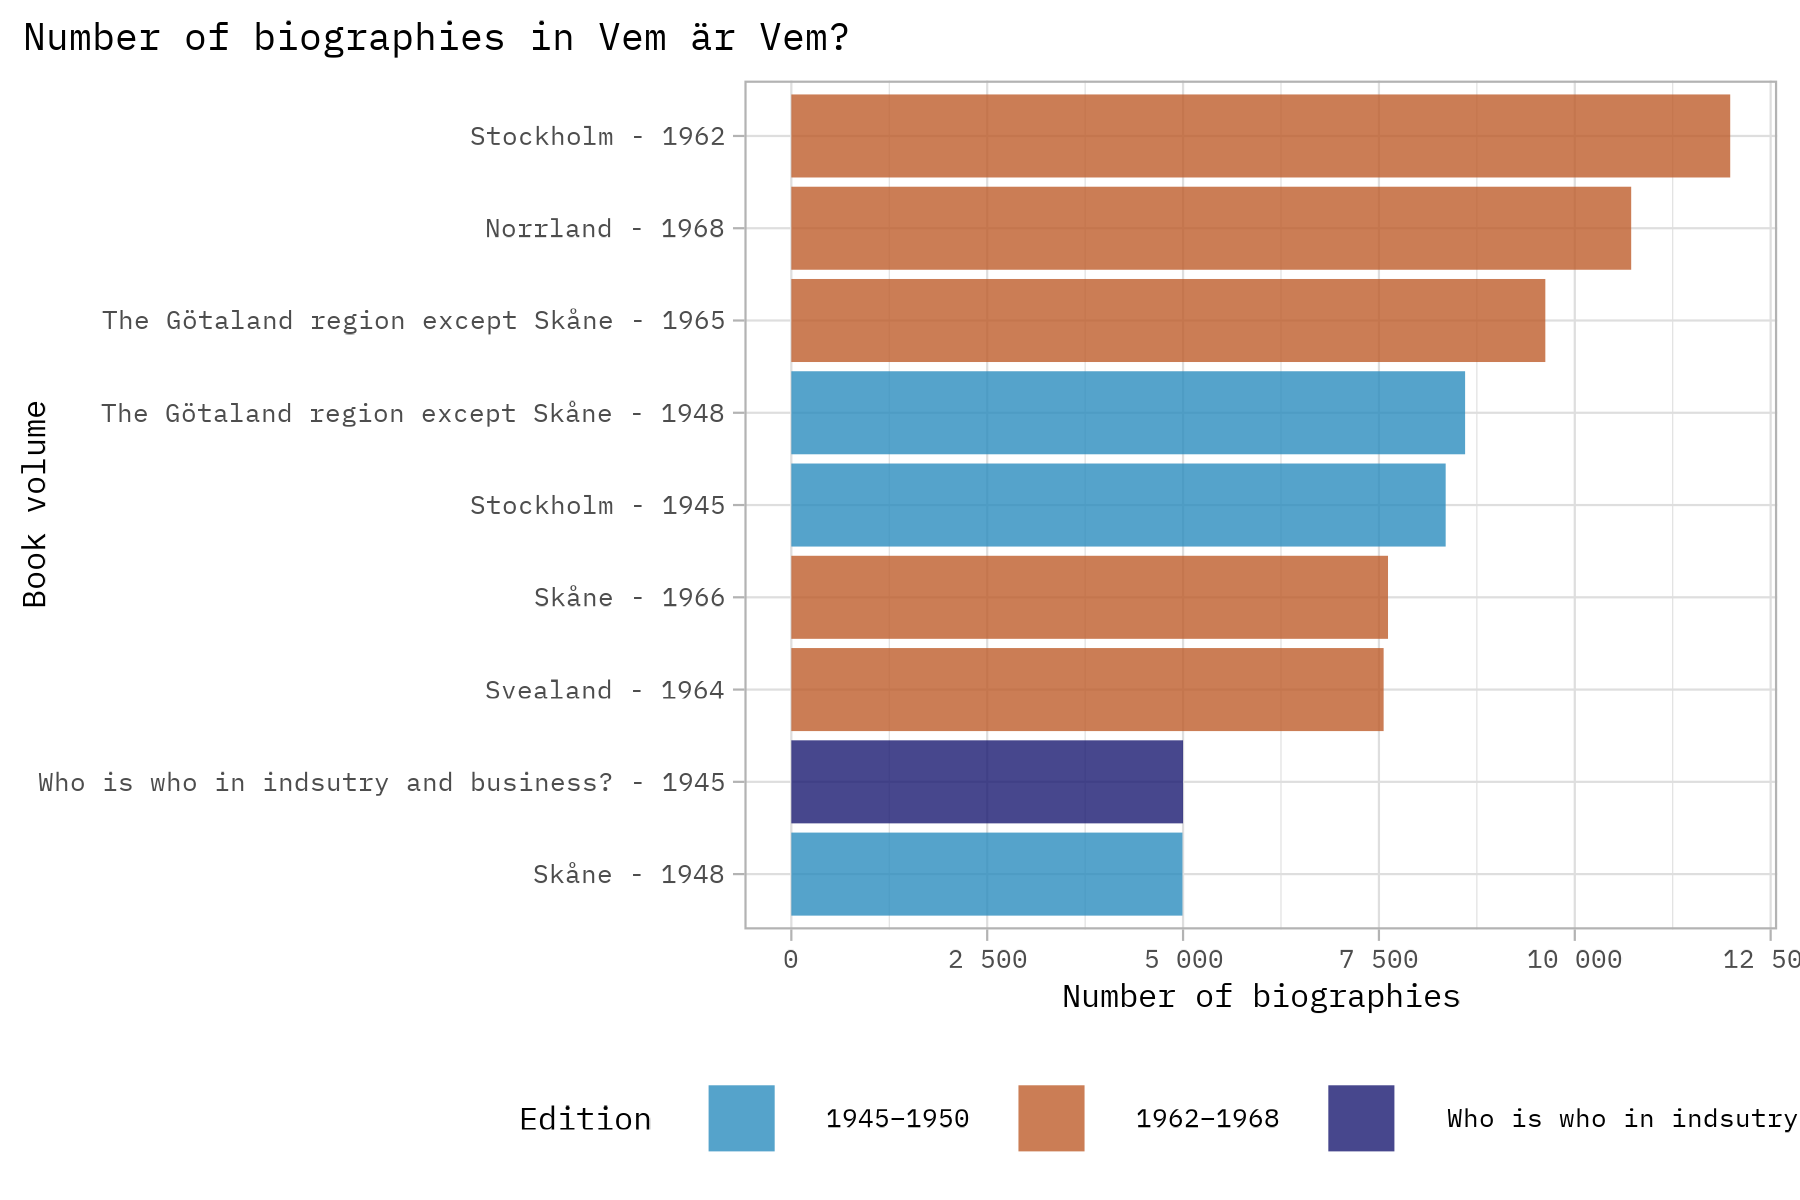
\includegraphics[width=5in,height=\textheight]{assets/who-is-who-volumes.png}

}

\caption{\label{fig-who-is-who-books}Number of biographies in each
volume of `Vem är Vem?'}

\end{figure}

In the context of economic and historical research, ``Vem är Vem?''
serves as a unique tool. By providing detailed biographies and career
information, it allows for an in-depth analysis of the human capital
that contributed to Sweden's economic and social evolution during the
mid-20th century.

The biographic information about the individuals in the dictionaries are
exemplified in Figure~\ref{fig-who-is-who-page}, which highlights the
life of chemist and metallurgist Karl Gustaf Lund.

\begin{figure}

{\centering 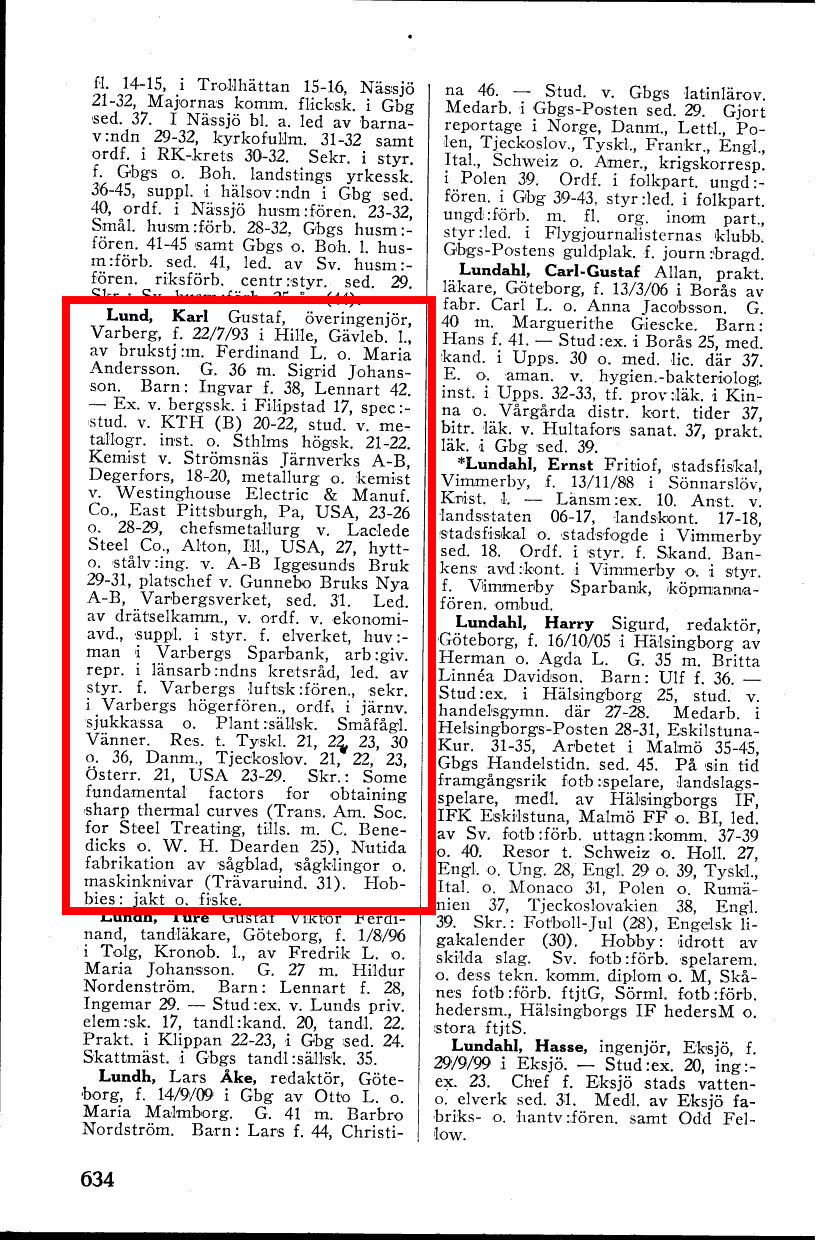
\includegraphics[width=2.72in,height=\textheight]{assets/vem_page.png}

}

\caption{\label{fig-who-is-who-page}A representative page of Vem är
Vem?, highlighting the biography of Karl Gustaf Lund}

\end{figure}

The fields include:

\begin{enumerate}
\def\labelenumi{\arabic{enumi}.}
\item
  \textbf{Education}: Lund's education at prestigious institutions such
  as the Royal Institute of Technology (KTH) indicates he had access to
  advanced technical knowledge. This level of education is critical for
  understanding the specialized skills that were necessary for
  innovation and advancement in electricity-related industries.
\item
  \textbf{Career Progression}: The text outlines Lund's career
  progression through various roles in metallurgy and chemical
  engineering. This trajectory can illustrate how individuals applied
  their education in practice, contributing to industrial development.
  Tracking such careers can provide insight into the professional
  development paths that were common and valued in the sector at the
  time.
\item
  \textbf{International Experience}: His experiences in the United
  States reflect the cross-border exchange of knowledge and skills. This
  can show how international experiences contributed to the domestic
  industry by importing new ideas and practices, which is a key aspect
  of human capital development.
\item
  \textbf{Leadership and Management}: Lund's leadership positions, such
  as chairmanships and advisory roles, imply a combination of technical
  expertise and managerial acumen. The ability to lead and innovate
  within companies is a significant aspect of human capital that drives
  industry growth.
\item
  \textbf{Research and Innovation}: The reference to his translated
  research work indicates an engagement with cutting-edge technology and
  knowledge creation. Such contributions are the tangible outputs of
  human capital in action, pushing the industry forward through
  innovation.
\item
  \textbf{Professional Networks}: His involvement with societies and
  associations suggests a networked professional community, which is
  essential for the diffusion of innovative ideas and practices. These
  networks are often where knowledge is exchanged, partnerships are
  formed, and collaborations are initiated.
\end{enumerate}

\hypertarget{industrial-catalogue}{%
\subsubsection{Industrial Catalogue}\label{industrial-catalogue}}

The Svensk Industrikalender from 1947, published by Sveriges
Industriförbund (Sweden's Industrial Association), is a comprehensive
directory of Swedish industrial firms. This calendar was issued annually
from 1918 to 2000 and contains information related to Swedish industry.
The 1947 edition available on the Project Runeberg website was digitized
in April 2012, sourced from the Centrum för Näringslivshistoria. The
calendar is believed to be under catalog protection but not copyright
{[}citation{]}.

It includes detailed information such as company names, locations,
nature of businesses, products, contact details, share capital, number
of employees, production values, establishment years, and key personnel
including managing directors and board members. This source is valuable
for studying the economic and industrial environment of post-war Sweden,
providing insights into corporate structures, industry distribution, and
business trends of that period.

A representative page is shown in Figure~\ref{fig-industry-calender}.

\begin{figure}

{\centering 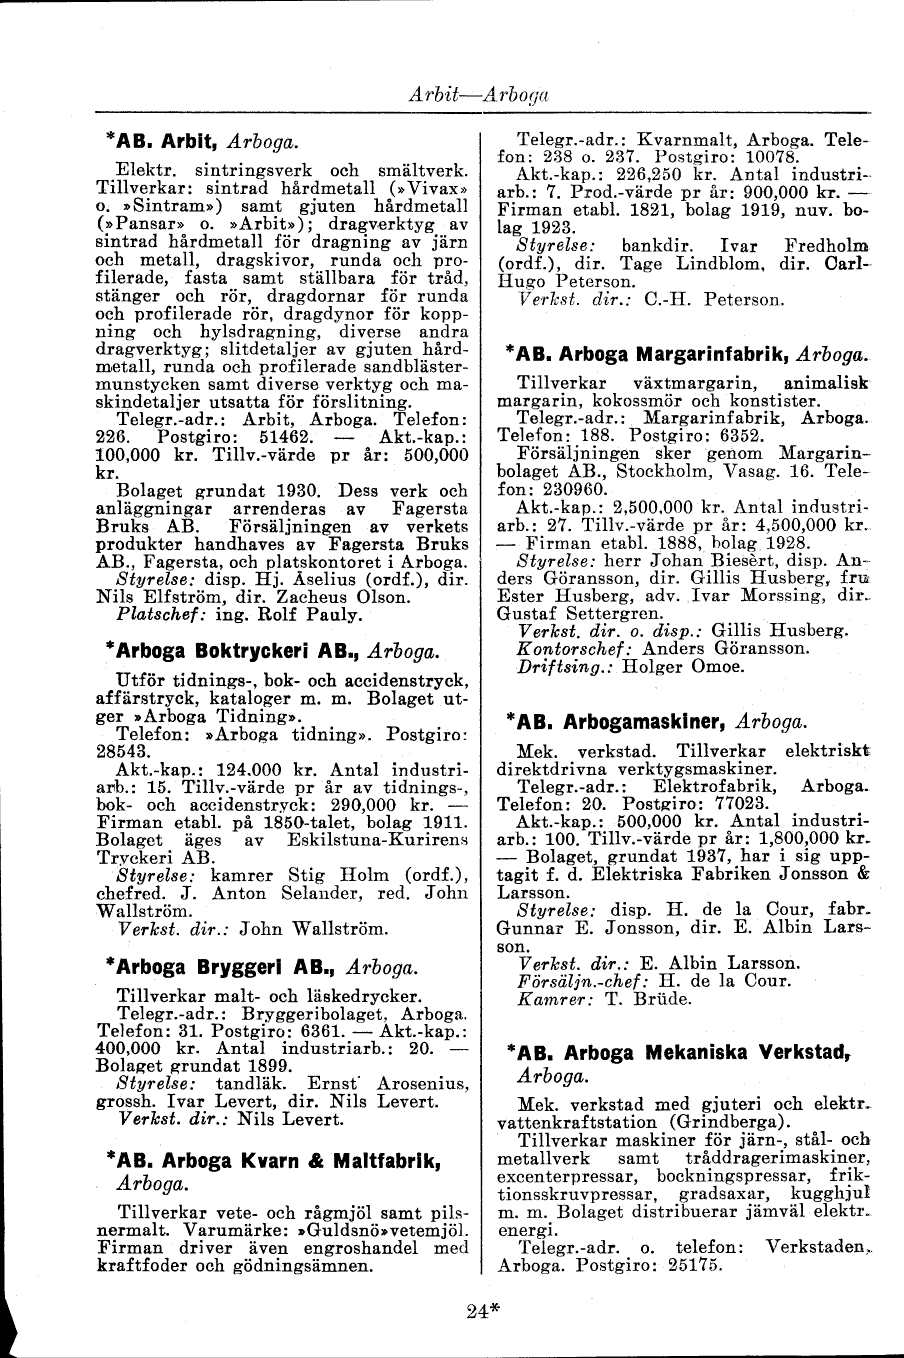
\includegraphics[width=6in,height=\textheight]{assets/svensk-industrikalender_1.png}

}

\caption{\label{fig-industry-calender}A page of the industry catalogue
from 1947}

\end{figure}

The common fields listed for each company entry in the catalogue are as
follows:

\begin{enumerate}
\def\labelenumi{\arabic{enumi}.}
\item
  \textbf{Company Name}: The name of the company is listed at the
  beginning of each entry, with an asterisk indicating membership of
  Sveriges Industriförbundet.
\item
  \textbf{Location/Town}: The town or location of the company, which in
  this case is \texttt{Arboga}.
\item
  \textbf{Description of Business}: A brief description of the company's
  main activities or products is provided.
\item
  \textbf{Products or Services Offered}: Specific items or services the
  company provides, such as types of machinery, tools, or materials.
\item
  \textbf{Contact Information}: This typically includes:

  \begin{itemize}
  \tightlist
  \item
    \textbf{Telegraph Address}: Listed as ``Telegr.-adr.'' indicating
    the address to which telegraphs are to be sent.
  \item
    \textbf{Telephone Number}: Listed as ``Telefon'' followed by the
    number.
  \item
    \textbf{Postal Code}: Mentioned as ``Postgiro'' or ``Postiro'' with
    corresponding numbers.
  \item
    \textbf{Bank Account}: Sometimes a bank account number or similar
    financial information is included.
  \end{itemize}
\item
  \textbf{Management and Key Personnel}: Names and titles of important
  figures in the company, such as the director (\texttt{Verkst.\ dir.}),
  board members, or founders.
\item
  \textbf{Financial Information}: Information about the financial aspect
  of the company, such as capital invested (\texttt{Akt.-kap.}) or
  turnover (\texttt{Tillv.-värde}).
\item
  \textbf{Establishment Details}: This includes the year of
  establishment and sometimes the history or lineage of the company's
  ownership or major changes.
\item
  \textbf{Address}: The full postal address, which may include a street
  name or a postbox number, indicated as \texttt{Postgiro}.
\end{enumerate}

This type of catalogue was commonly used for business-to-business
interactions and can be considered an early form of networking resource,
allowing companies to find suppliers, customers, and partners.

\hypertarget{data-collection-strategy}{%
\subsection{Data collection strategy}\label{data-collection-strategy}}

In order to analyze both the biographical dictionaries and industrial
catalogue, we need to bend the text into a machine readable structure.
This process is relatively complicated. It involves breaking each
component of the source up (e.g.~each biography or company record),
extracting the pertinent information from each record, storing each
value with its associated key, and then saving this information in a way
that is easy to analyze and aggregate.

The simplified process is laid out in
Figure~\ref{fig-data-collection-process}. The underlying code can be
found on the GitHub repo linked at on the first page of this paper. I
detail the third step, structuring the records, in the section below,
and the remainder of the steps in the appendix.

\begin{figure}

{\centering 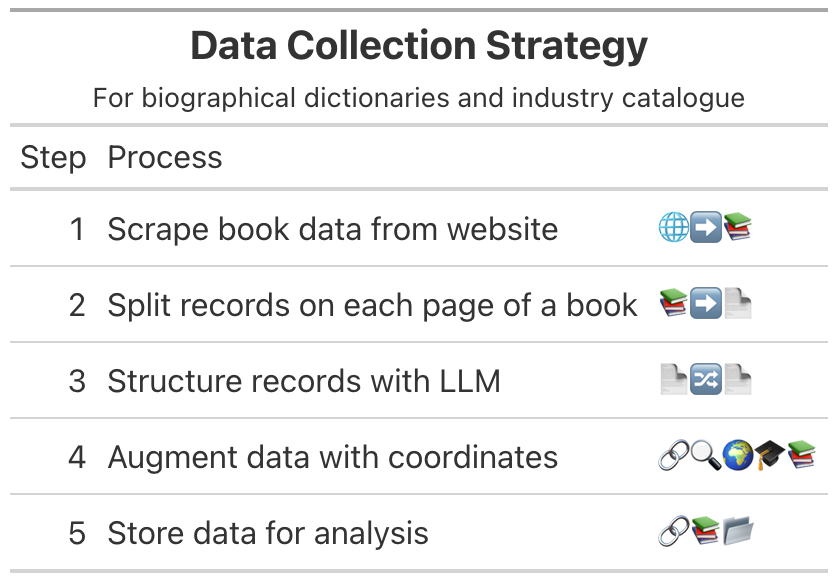
\includegraphics[width=5in,height=\textheight]{assets/data-collection-process.png}

}

\caption{\label{fig-data-collection-process}Data collection process
steps}

\end{figure}

Prior to the advent of Large Language Models (LLMs), this was a task
that required a large number of human hours to complete, either putting
the information into an excel sheet by hand, or writing rules to extract
the information from the text. The first approach limits the number of
observations a researcher can collect on her own, and the second
approach quickly turns into the first.

Due to the number of abbreviations, acronyms and contractions (for
example, \texttt{Gävleb.\ l.} is the contraction of \emph{Gävleborg län}
or Gävleborg county in Figure~\ref{fig-who-is-who-page}), while it might
be possible to take a simple rules based approach to replacing these
contractions with their complete Swedish text, and then looking for
specific terms relating to each piece of information, the number of
rules soon balloons to an unreasonable figure. Writing a rule for every
case necessitates as much human involvement as would be required to
manually structure the information - the first approach.

However, with the rapid advancements in LLM technology in the previous
five years, and poplular adoption of these tools through Chat-GPT and
Microsoft's integration of GPTs into their products in the previous
year, new tools mean this manual workload can be avoided to a large
extent.

I make use of the backed of Chat-GPT, a model called GPT-3.5-turbo from
OpenAI to structure the information from the dictionaries and catalogue
into a JSON format that I can analyse, step 3, as shown in
Figure~\ref{fig-data-collection-process}.

By passing the text to the LLM, along with some context about what the
model is being given, the model can behave like a skilled research
assistant, reading the records, searching for the specific pieces of
information requested, and outputting a structured file containing the
information that we seek.

\hypertarget{intuitive-explanation-of-llms-contextual-understanding}{%
\subsubsection{Intuitive explanation of LLMs contextual
`understanding'}\label{intuitive-explanation-of-llms-contextual-understanding}}

The GPT-3.5-turbo model which I make use of is a LLM which has been
trained on all of Wikipedia and Wikidata, among other training material.
These two sources contain the same information, but in a different
format, as shown in the adapted extracts below. As the base model that
is pre-trained to predict the next token on this kind of data, it has
developed the ability though repeated exposure to this kind of
biographic data to produce structured information from free text, and
likewise construct natural sounding text from pieces of structured
information.

\emph{Jonas Wenström (4 August 1855 in Hällefors -- 22 December 1893 in
Västerås) was a Swedish engineer and inventor, who in 1890 received a
Swedish patent on the same three-phase system independently developed by
Mikhail Dolivo-Dobrovolsky. He studied at Uppsala University.}

\begin{longtable*}{ll}
\caption*{
{\large Wikidata information about Swedish inventor \textbf{Jonas Wenström}}
} \\ 
\toprule
Key & Value \\ 
\midrule\addlinespace[2.5pt]
Name & Jonas Wenström \\ 
Birth Date & 1855-10-04 \\ 
Death Date & 1893-12-21 \\ 
Occupations & Engineer, Inventor \\ 
Education & Uppsala University \\ 
\bottomrule
\end{longtable*}

\hypertarget{example-of-structured-biographic-text}{%
\subsubsection{Example of structured biographic
text}\label{example-of-structured-biographic-text}}

Following this process of structuring the records into a format with
specified keys and values, I augment the data by geocoding locations in
order to analyse geographic paths of individuals in the sample, and
geographic clusters of firms.

Below I show the output of the data collection process, where the
biographical dictionary entry on Swedish engineer and power station
manager Axel Verner Nordell is shown in Figure~\ref{fig-axel} and some
of the extracted information along with the geocoded coordinates are
shown in Table~\ref{tbl-axel}.

\begin{figure}

{\centering 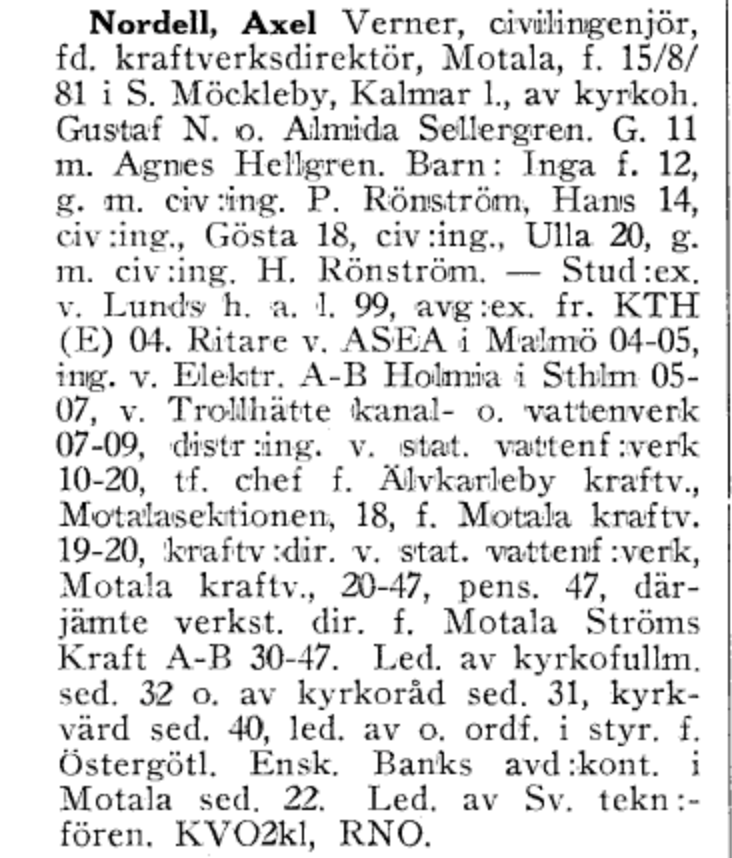
\includegraphics[width=3in,height=\textheight]{assets/axel.png}

}

\caption{\label{fig-axel}Raw information about Swedish engineer and
power station manager Axel Verner Nordell}

\end{figure}

\newpage{}

\hypertarget{tbl-axel}{}
\begin{longtable}{ll}
\caption{\label{tbl-axel}Extracted information about Axel Verner Nordell }\tabularnewline

\caption*{
{\large Selected collected information about Swedish engineer and power station manager\textbf{Axel Verner Nordell}}
} \\ 
\toprule
Key & Value \\ 
\midrule\addlinespace[2.5pt]
full\_name & Nordell, Axel Verner \\ 
location & Motala, Östergötland \\ 
occupation & Civilingenjör, kraftverksdirektör \\ 
birth\_date & 15/08/1881 \\ 
birth\_place & S. Möckleby, Kalmar \\ 
birth\_parents & Gustaf N. and Amanda Seillergren \\ 
birth\_latitude & 56.35646300000001 \\ 
birth\_longitude & 16.420155 \\ 
education\_degree & Studentexamen \\ 
education\_year & 1899 \\ 
education\_institution & Lunds högre allmänna läroverk \\ 
education\_latitude & 55.7046601 \\ 
education\_longitude & 13.1910073 \\ 
\bottomrule
\end{longtable}

\hypertarget{clustering-of-firms-and-classification-of-occupations}{%
\subsection{Clustering of firms and classification of
occupations}\label{clustering-of-firms-and-classification-of-occupations}}

The next task involved grouping the firms from the catalogue and then
classifying each individual in the biographical dictionaries into a
particular occupation in order to track the trends in the labour market.

For both of these tasks, I lent on the tools of text embeddings, and a
combination of unsupervised machine learning and advanced language
processing techniques. I made use of a text embedding model trained on
Swedish language text by the Royal Library
\textcite{bert-base-swedish-cased}. It is an adaptation of the
breakthrough BERT model, introduced by Google Research in 2018
{[}citation{]}. The advantage of this model is that it has been trained
on a selection of Swedish data, including books, news reports, and
internet forums. Hence it is able to score the similarity of Swedish
business descriptions and occupational titles.

Text embeddings are effective for clustering because they capture
semantic meaning rather than relying on surface-level features like
character composition. For example, while ``steam engine'' and ``power
station'' are different in characters and literal meaning, they are
semantically related in the context of industrial machinery and energy
production. Text embeddings transform these phrases into numerical
vectors that reflect this semantic similarity. When applied to
clustering, this means that items with similar meanings, even if their
literal expressions differ, are grouped together based on the contextual
and conceptual similarities encoded in their embeddings. This capability
makes text embeddings particularly powerful for organizing and
categorizing text data in a way that aligns with human understanding and
interpretation. {[}citation{]}

For grouping firms, I used the k-means clustering algorithm, an
unsupervised learning method, to categorize firms into 20 distinct
categories. This algorithm works by partitioning the data into k
distinct clusters based on features (in this case, text embeddings
derived from company descriptions). {[}citation{]}

The result of this classification is visible in
Figure~\ref{fig-density-ridges}, which shows the number of firms founded
each year by category from the industrial catalogue. The clusters are
ordered by peak year for foundation. We see that Breweries, malt and
soft drink factories are some of the first established industrial
businesses, along with book printing and publishing. At the bottom of
the figure, it is evident that electrical appliance and mechanical
machinery manufacturers, as well as firms in the chemical and
pharmaceutical industries have the greatest number of firms founded in
the years just prior to 1947, when our industrial firm catalogue is
produced.

\begin{figure}

{\centering 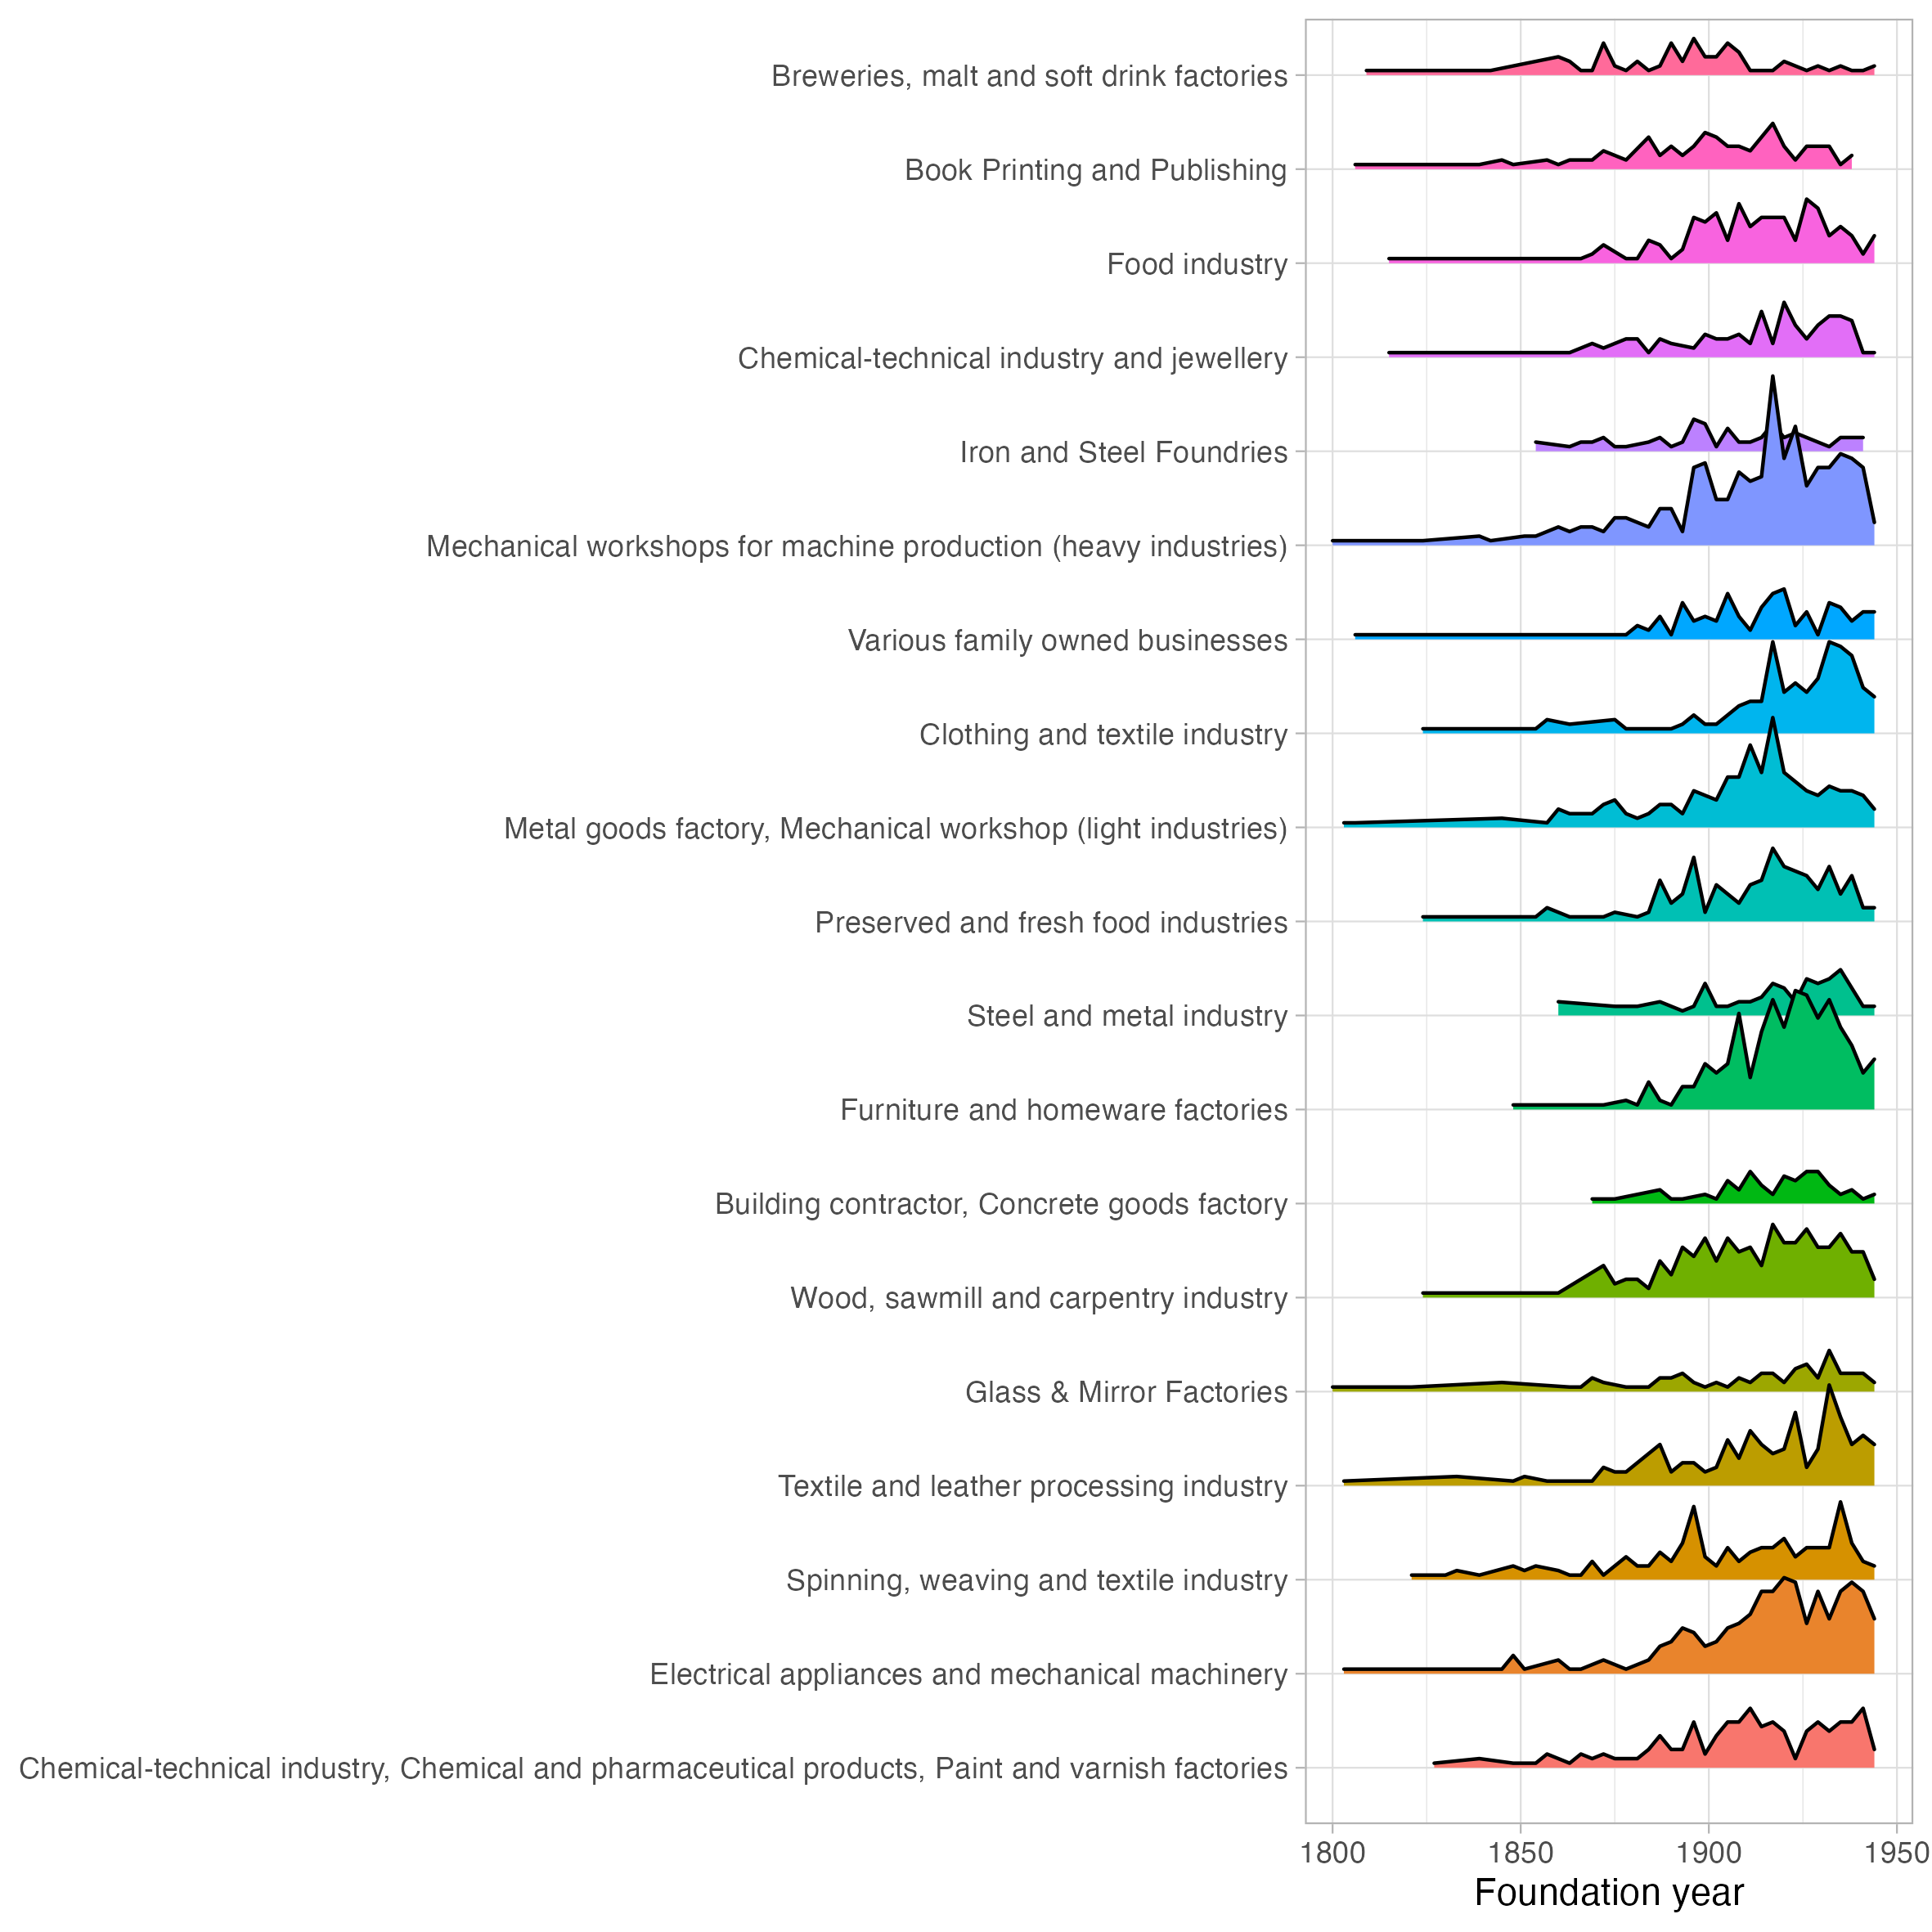
\includegraphics[width=5in,height=\textheight]{assets/geom_density_ridges.png}

}

\caption{\label{fig-density-ridges}Density plot showing the foundation
year of the firms in the 20 categories derived from the business
descriptions}

\end{figure}

In classifying occupations, I utilized the KB BERT model to create
sentence embeddings for both the titles in the three-digit Historical
International Standard Classification of Occupations (HISCO) schema and
for each occupation in my biographical dictionary data. These embeddings
were then projected into a 364-dimensional vector space. For each
occupation, I determined the closest HISCO code in this vector space
based on cosine distance, a measure of similarity without a specific
unit. I established a threshold for this distance to ensure that the
occupation was `close enough' to the corresponding HISCO code, setting
it to a level where 85\% of occupations received a HISCO code. While
somewhat arbitrary, this approach allowed for a contextually relevant
classification of occupations, drawing on the advanced language
understanding capabilities of the KB BERT model.

\hypertarget{what-does-the-industrial-calendar-tell-us-about-industrial-firms-in-sweden-in-1947}{%
\subsection{What does the industrial calendar tell us about industrial
firms in Sweden in
1947?}\label{what-does-the-industrial-calendar-tell-us-about-industrial-firms-in-sweden-in-1947}}

{[}Explain that we see forestry and wood business in rural areas and the
North of Sweden (purple), we see mechical workshops in modern day Skåne
(pink), we see a cluster of furniture factories and home goods factories
in central Southern Sweden, and a cluster of electrical appliance and
mechanical machinery stores around Stockholm. Note that these clusters
don't show all firms of one type, but the location of firms by
geographic cluster, and the most common firm in that geographic cluster
- makes it easier to see than many dots overlapping.{]}

\begin{figure}

{\centering 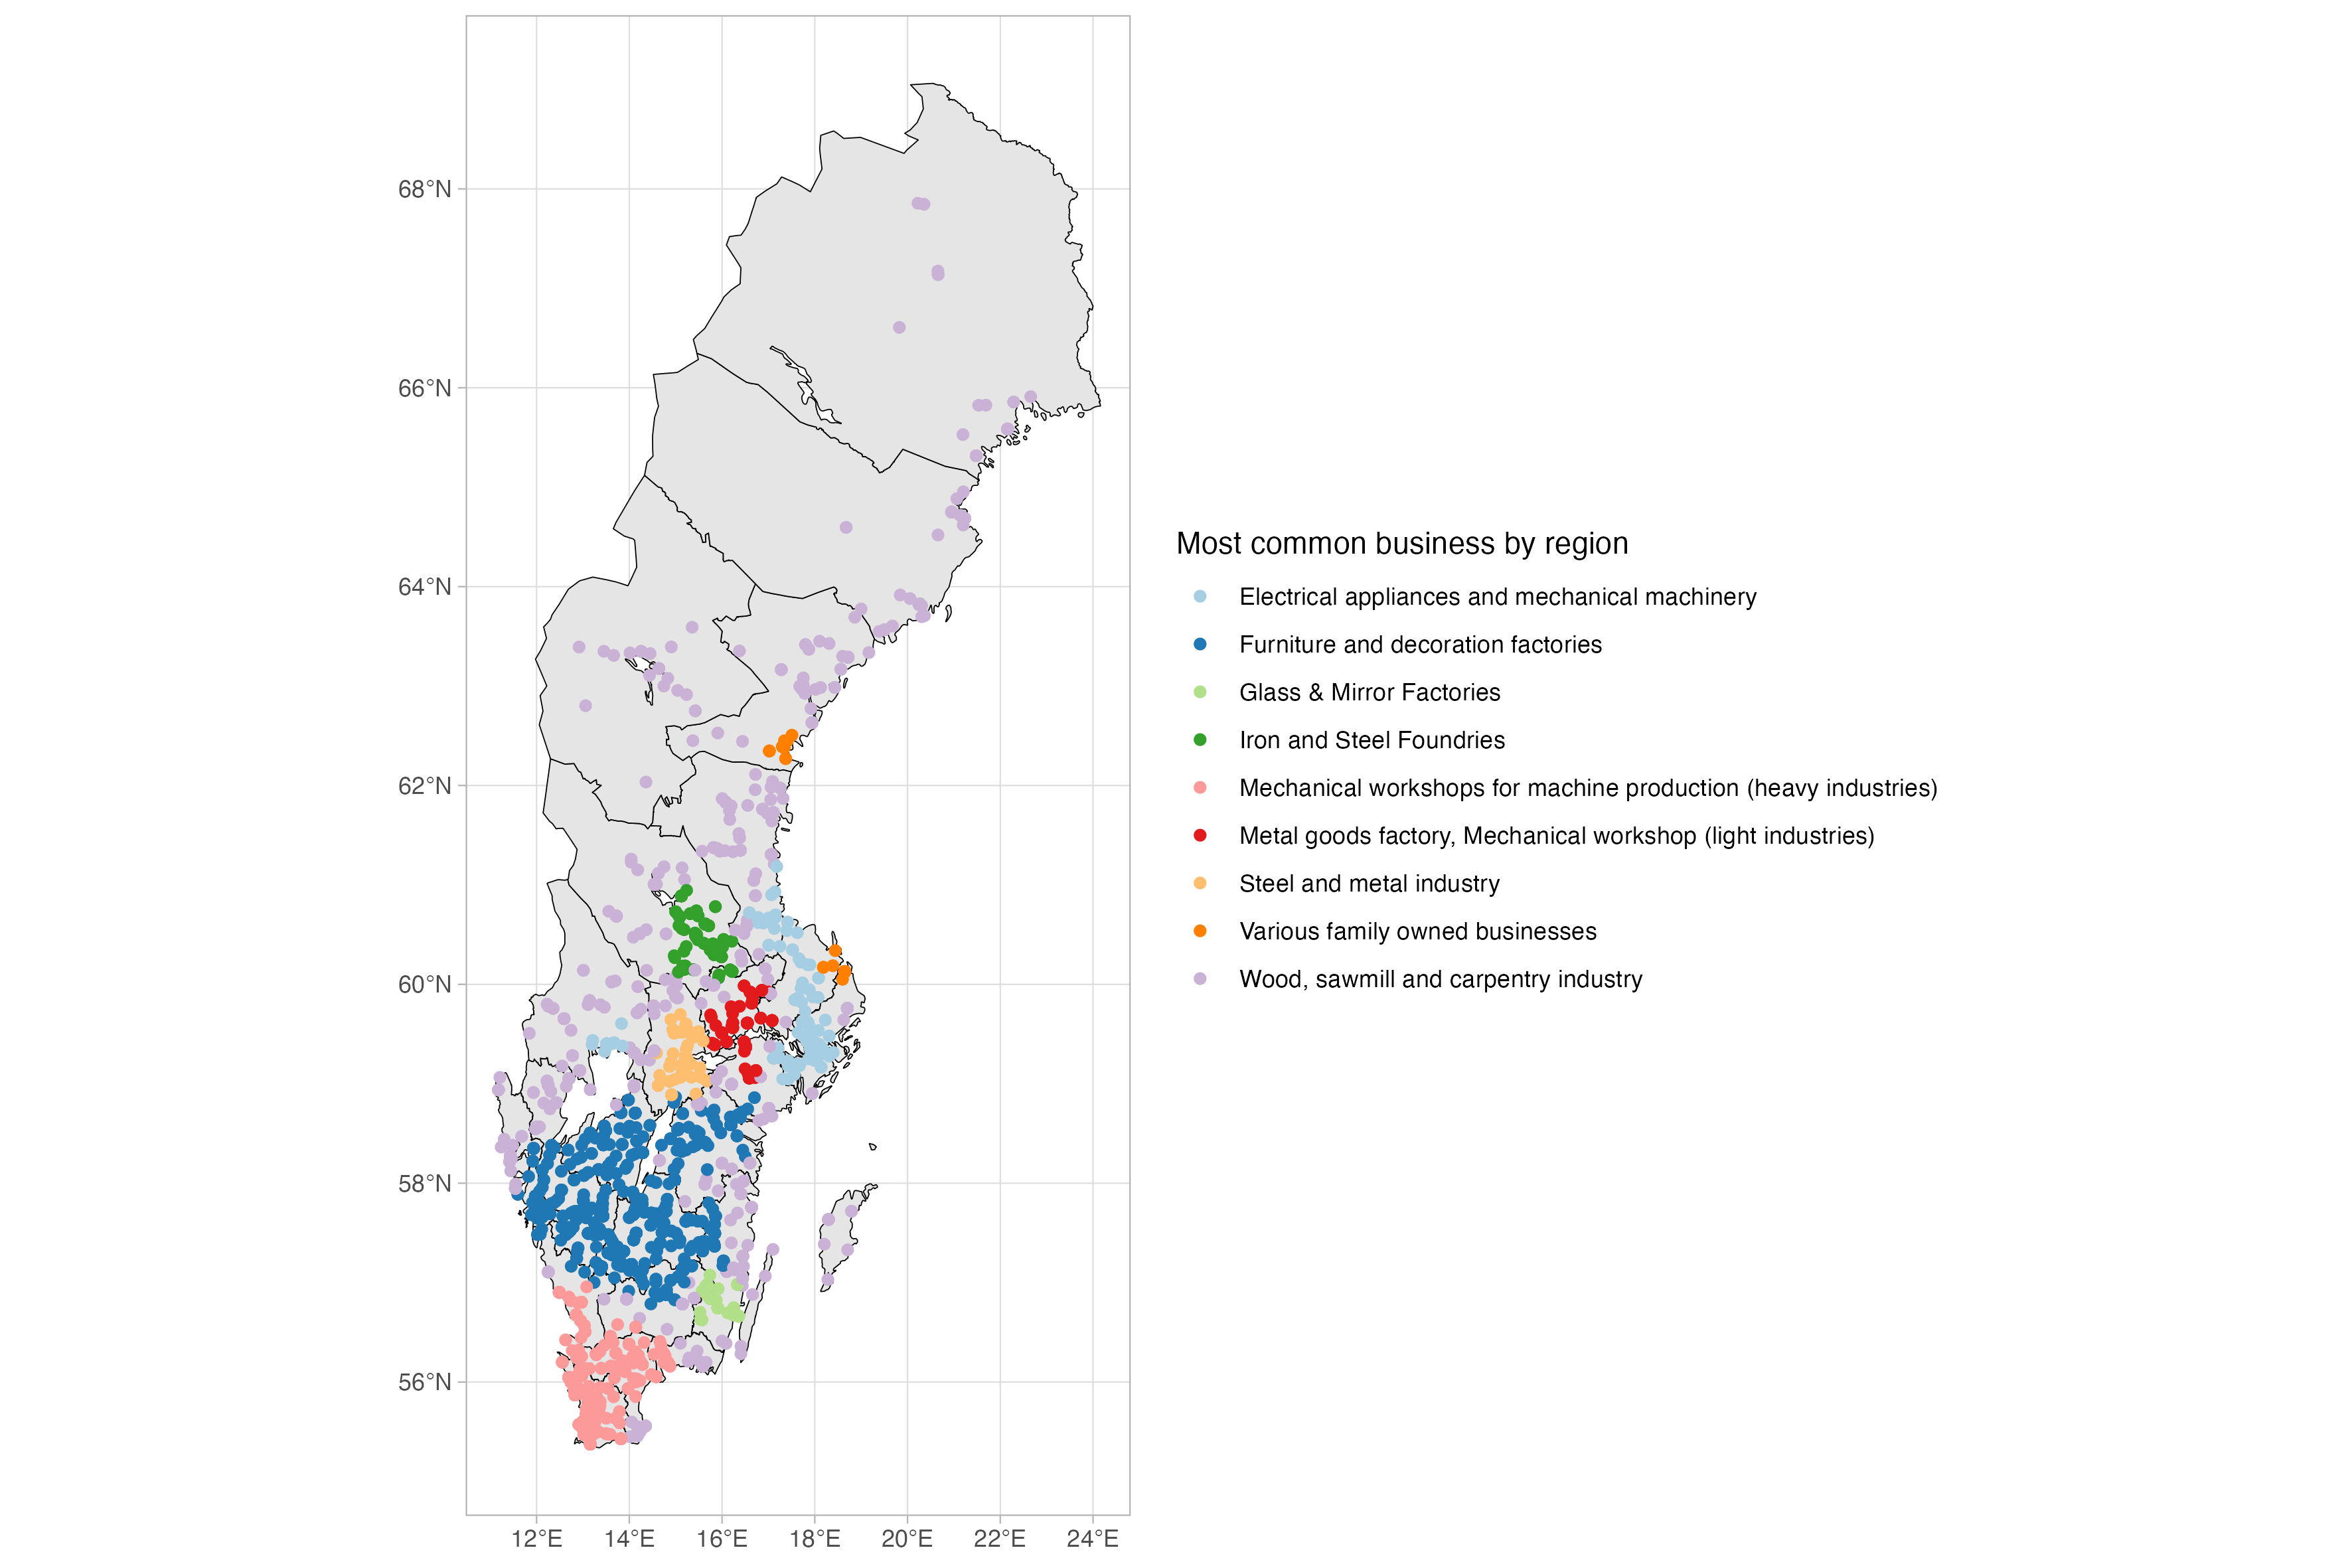
\includegraphics[width=8.5in,height=\textheight]{assets/map_most_common_businesses.png}

}

\caption{\label{fig-common-businesses}Map of the geographic clusters of
businesses by most common business type}

\end{figure}

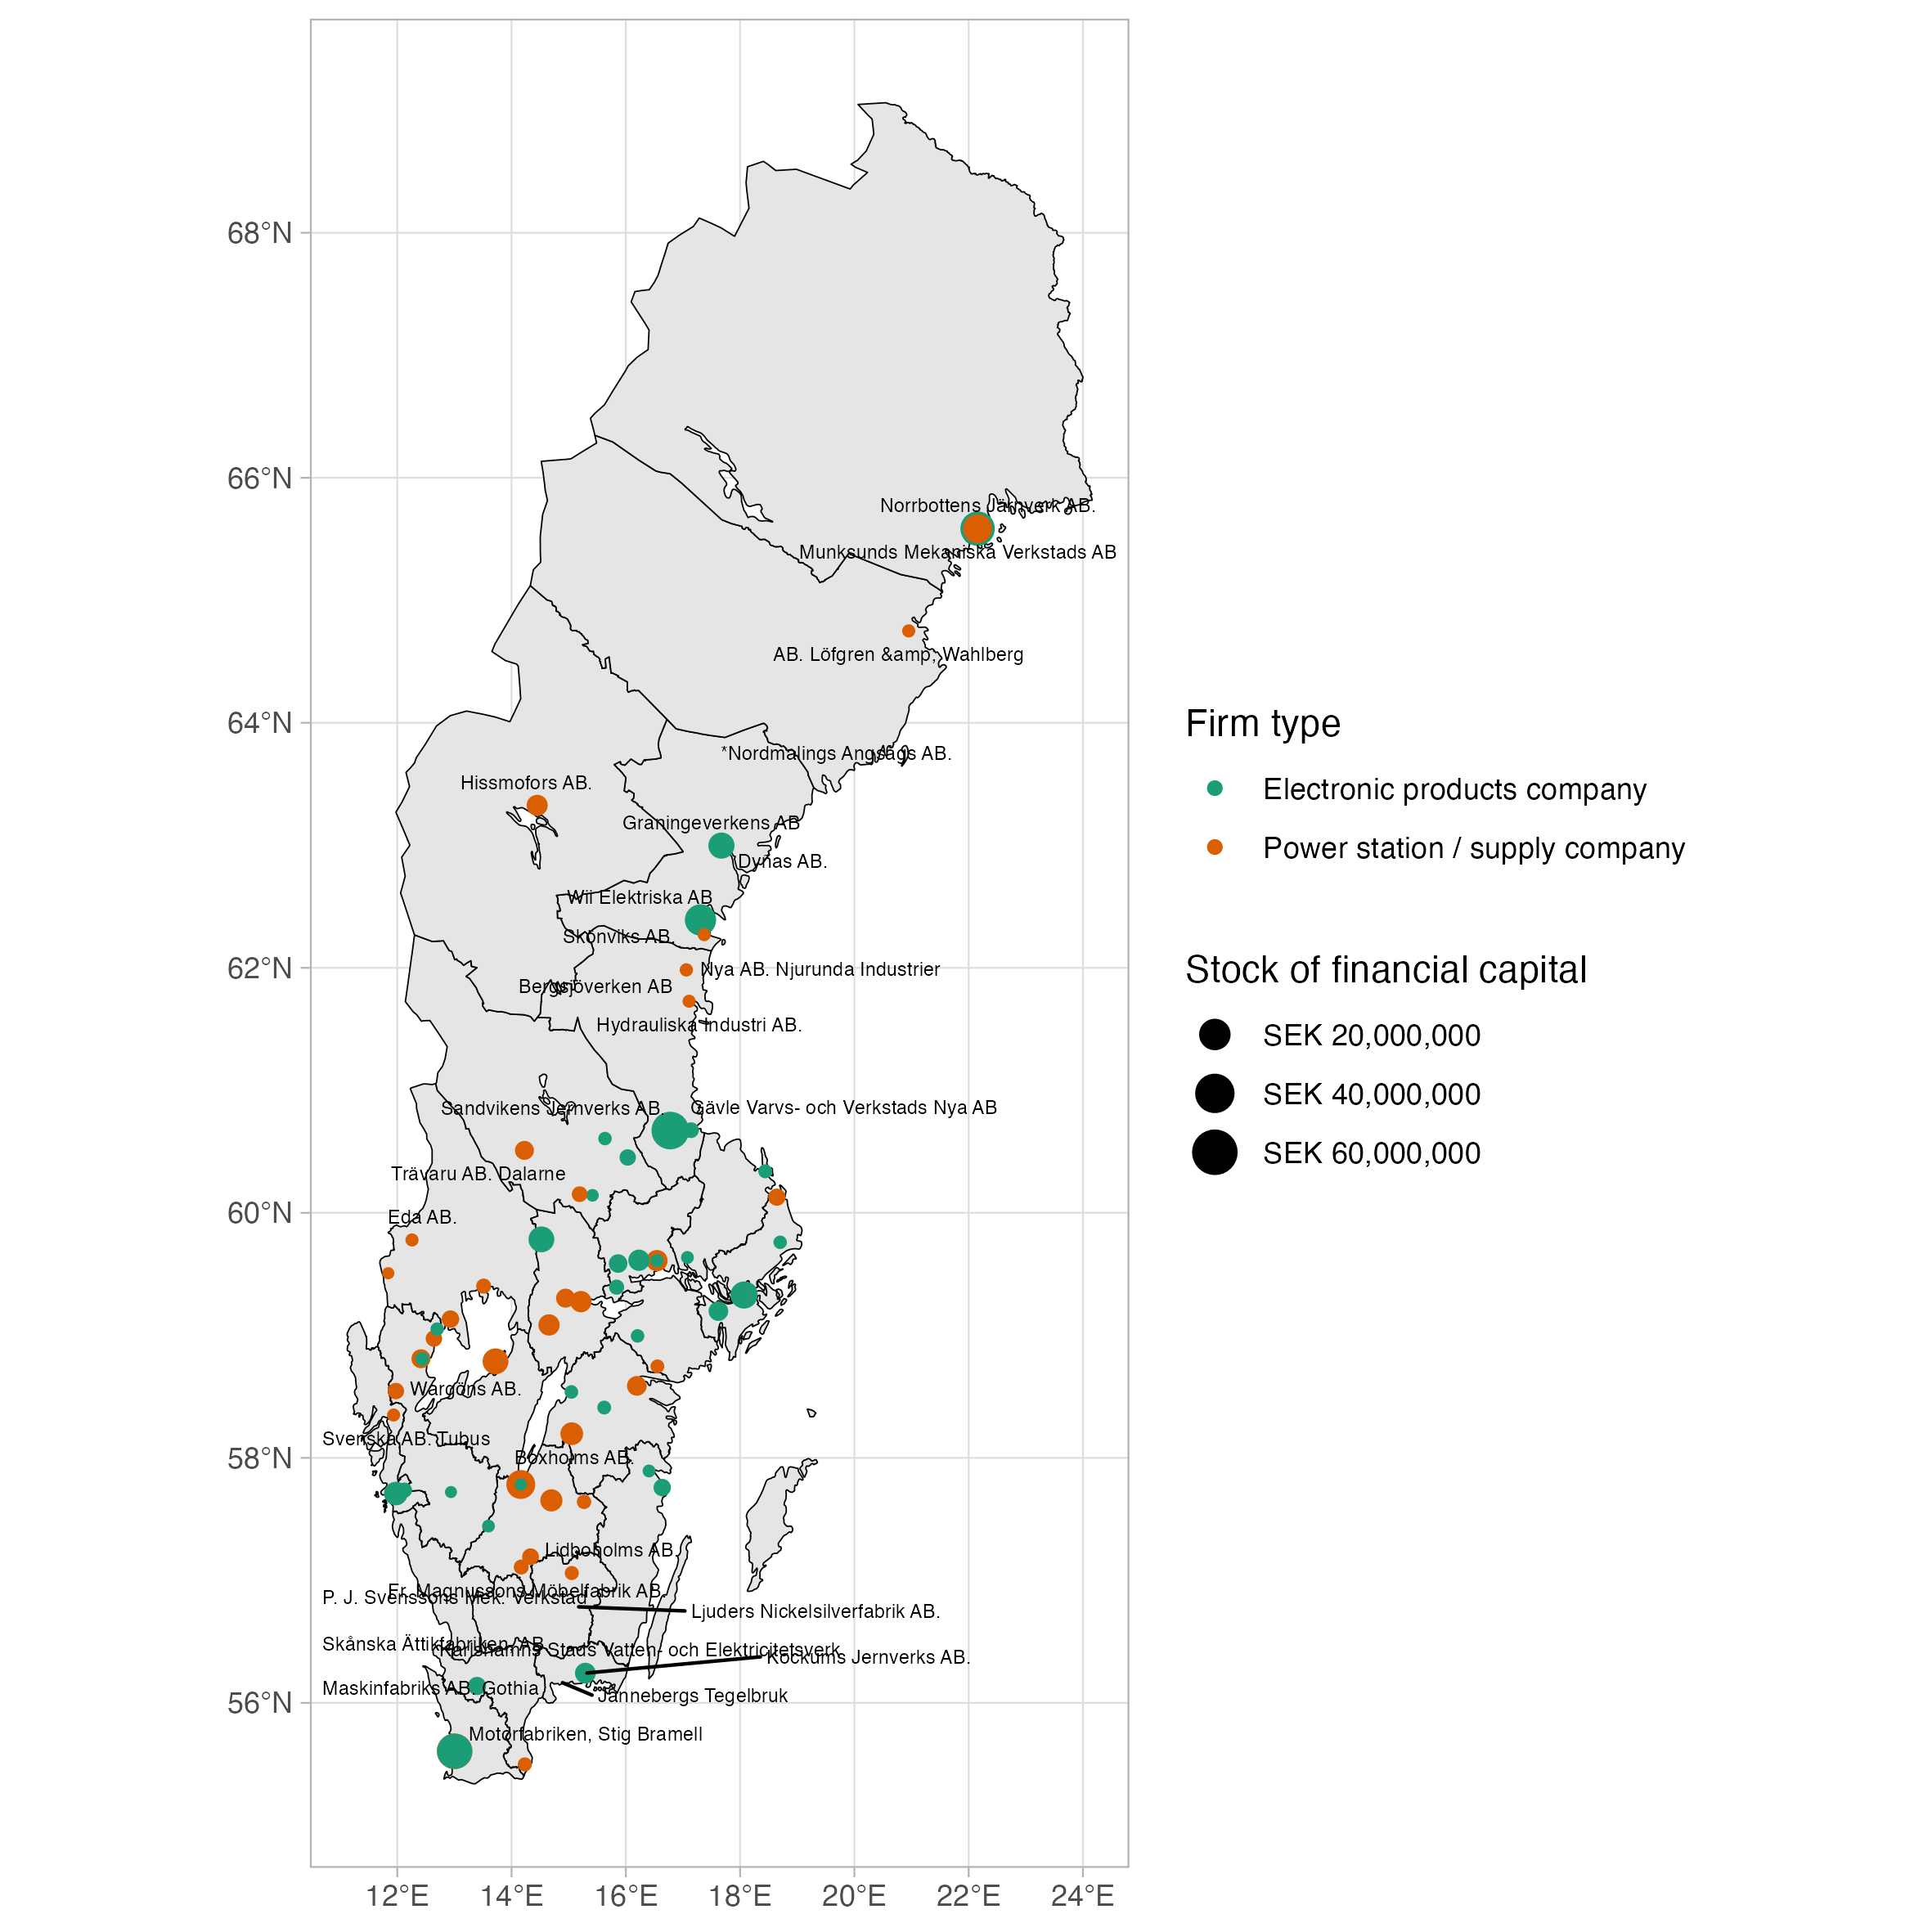
\includegraphics{assets/map_of_electricity_related_businesses.png}

{[}In this map, we show two kinds of firms; firms taht make electronic
products, and firms that produce power or supply power stations with
equipment. We can see that electronic products companies are clustered
near the large population centers of Stockholm, Gothenburg and Malmö.
There are many power stations in central Southern Sweden that make use
of hydropower, and firms near them that supply equipment for these power
stations.{]}

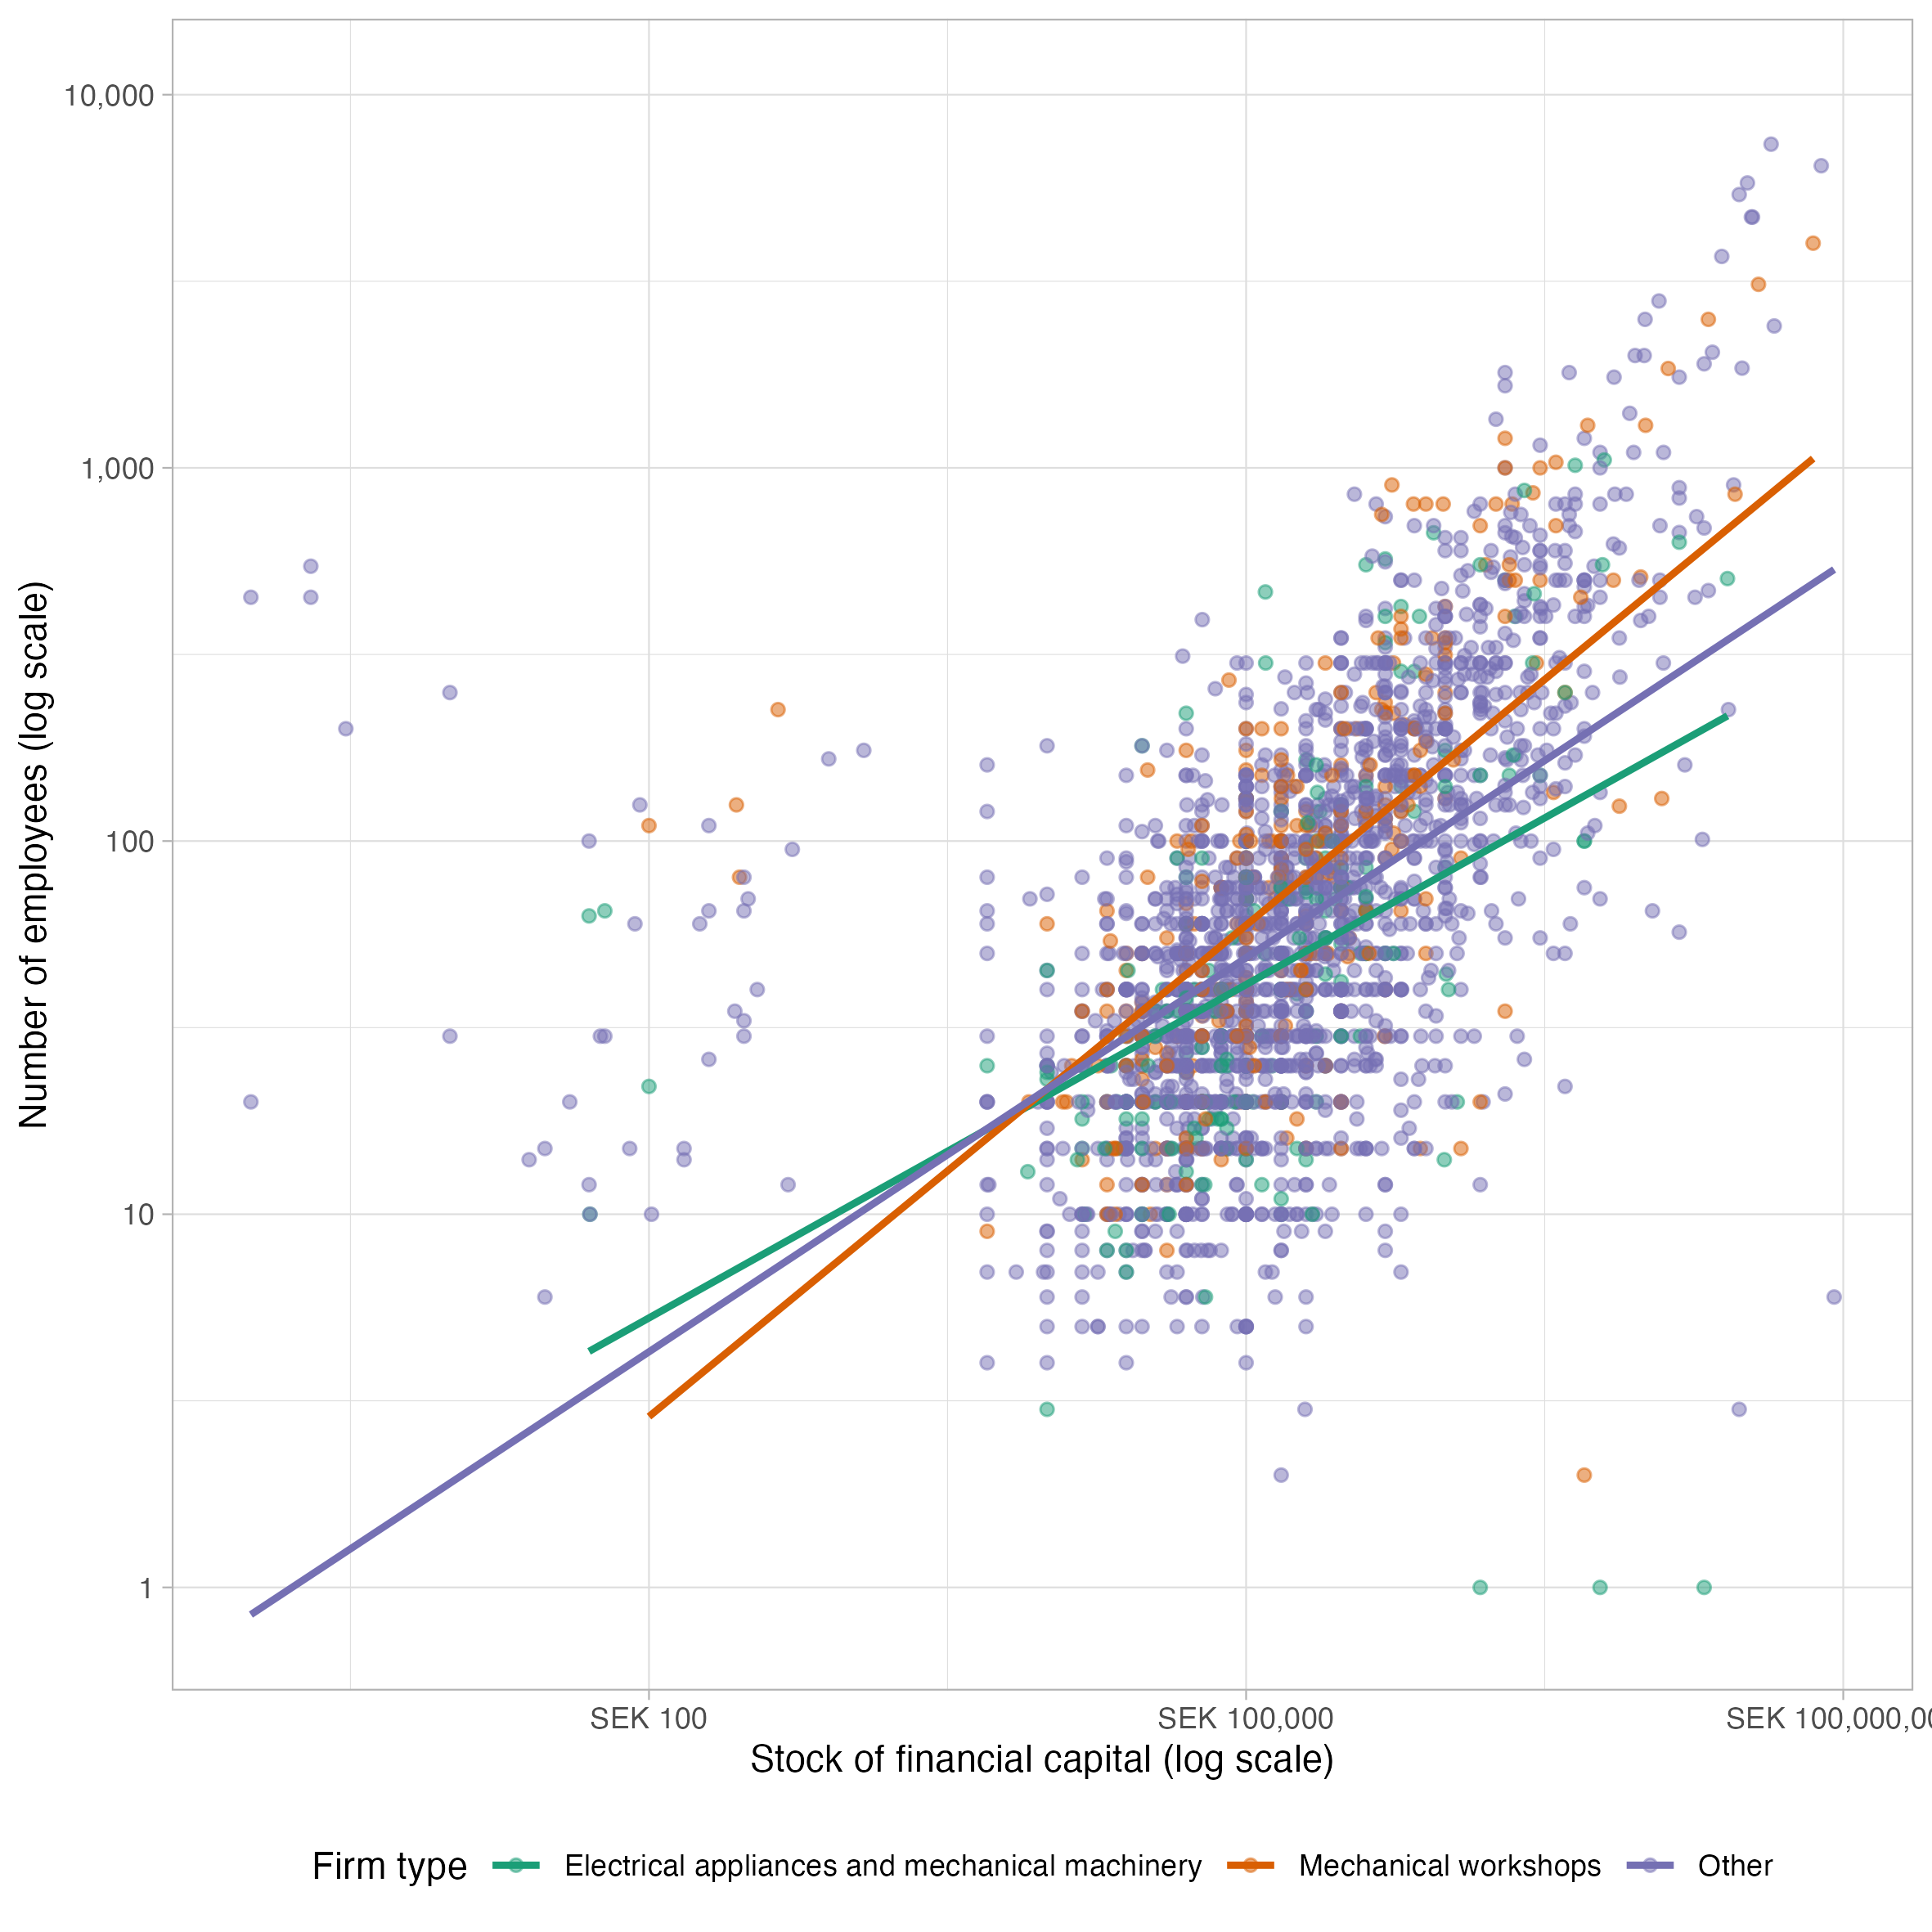
\includegraphics{assets/capital_vs_employees.png}

{[}Here we show that mechanical workshop firms are relatively labour
intensive, while electrical appliance and machinery producing firms are
relatively capital intensive, compared to all other firms (in purple){]}

\hypertarget{what-can-we-learn-from-the-who-is-who-biographies}{%
\subsection{What can we learn from the Who is Who?
biographies?}\label{what-can-we-learn-from-the-who-is-who-biographies}}

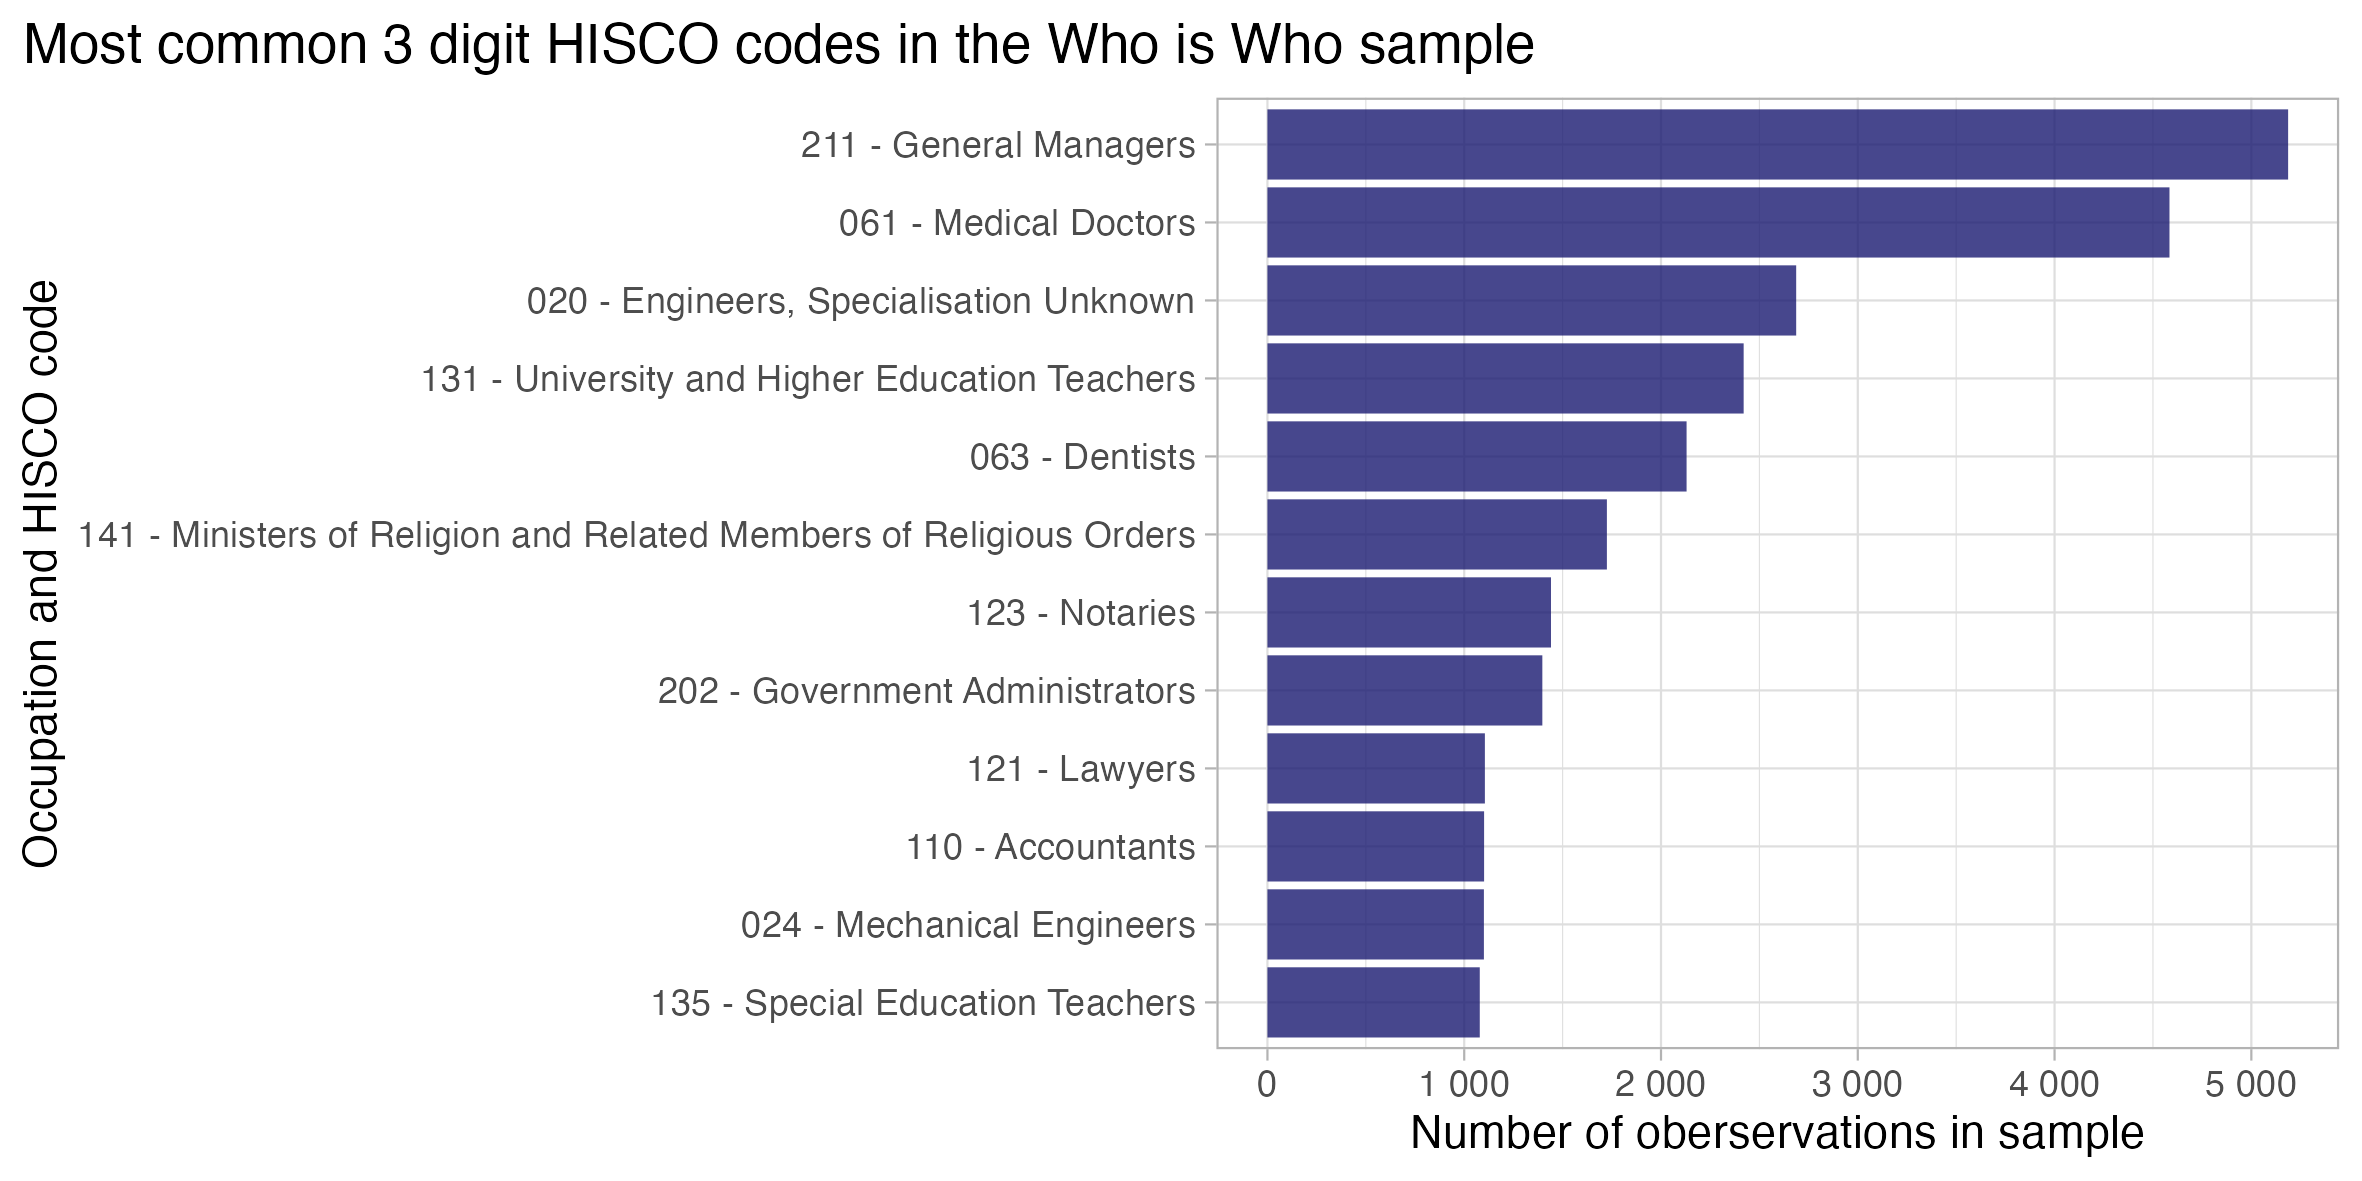
\includegraphics{assets/hisco_counts.png}

{[}We can show that of those in our sample, a great deal are general
managers of firms, as well as doctos, dentists, teachers and priests.
Engineers make up a large other component.{]}

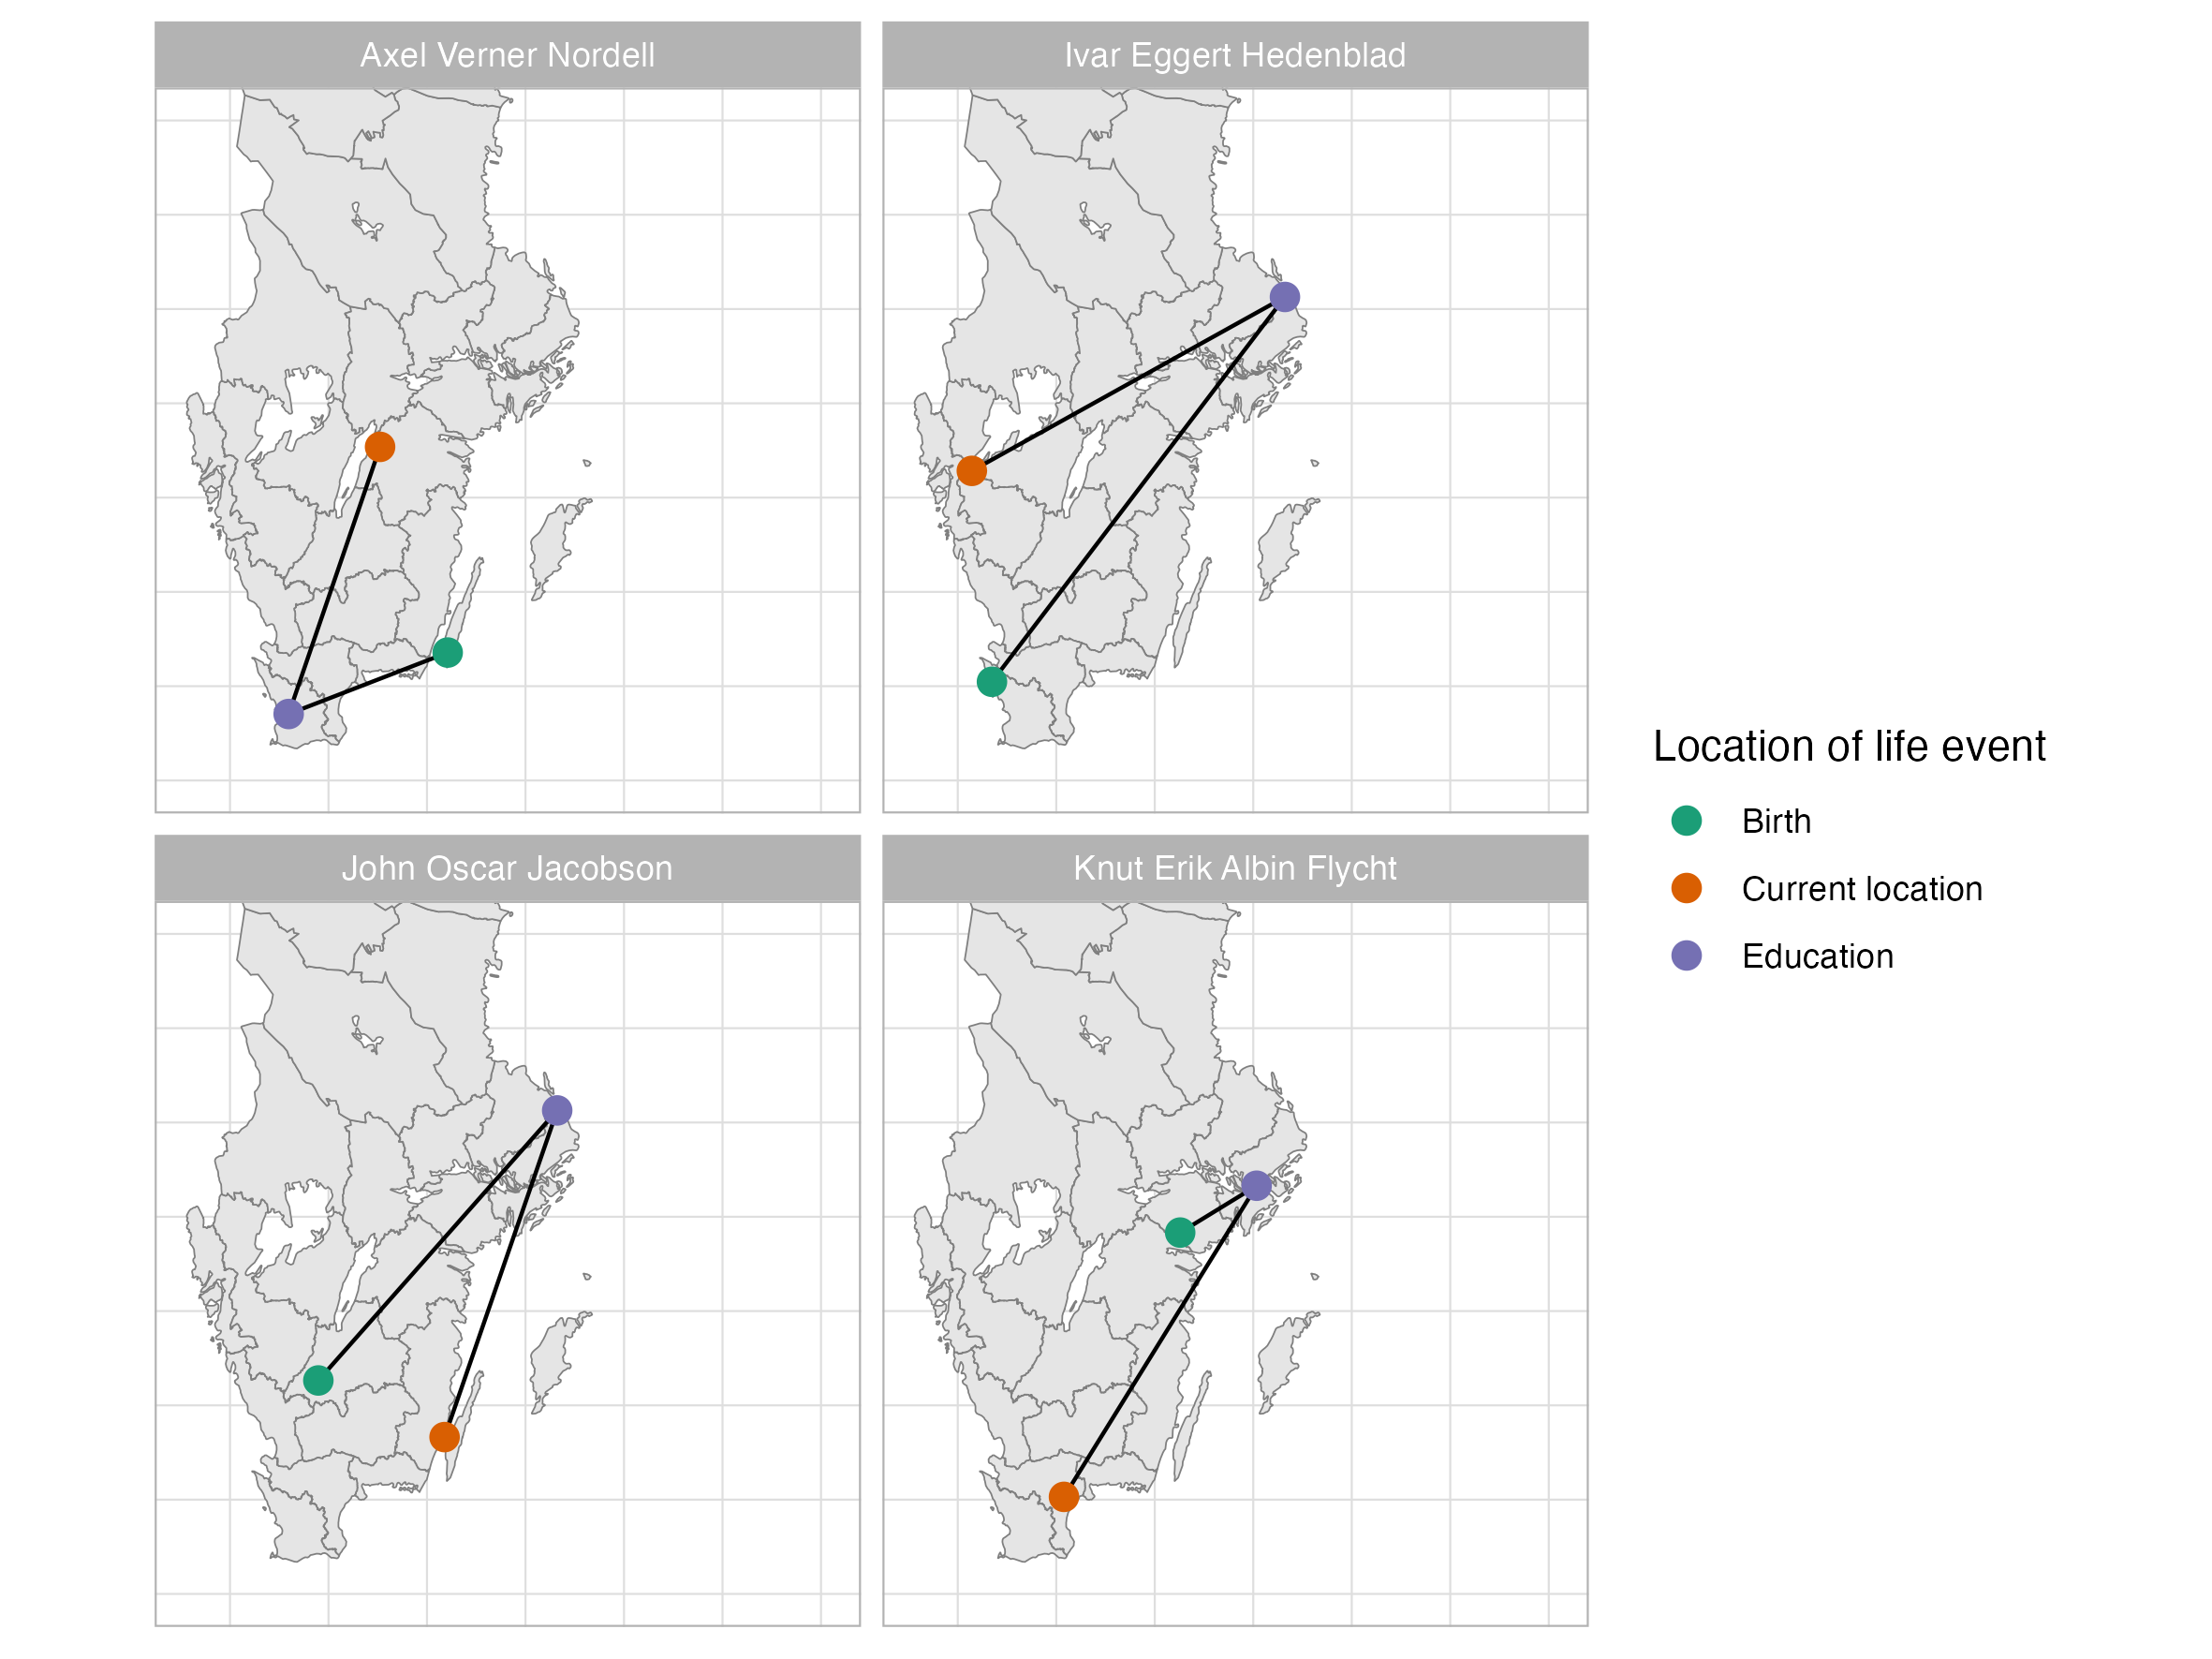
\includegraphics{assets/eee_map.png}

{[}We can show that electrical and electronic engineering technicians
move the furthest from the birthplace to their places of education, and
further still from their place of education to their current location.
Not the case that local lads were filling the roles for skilled workers
in these new occupations - kinda interesting!{]}

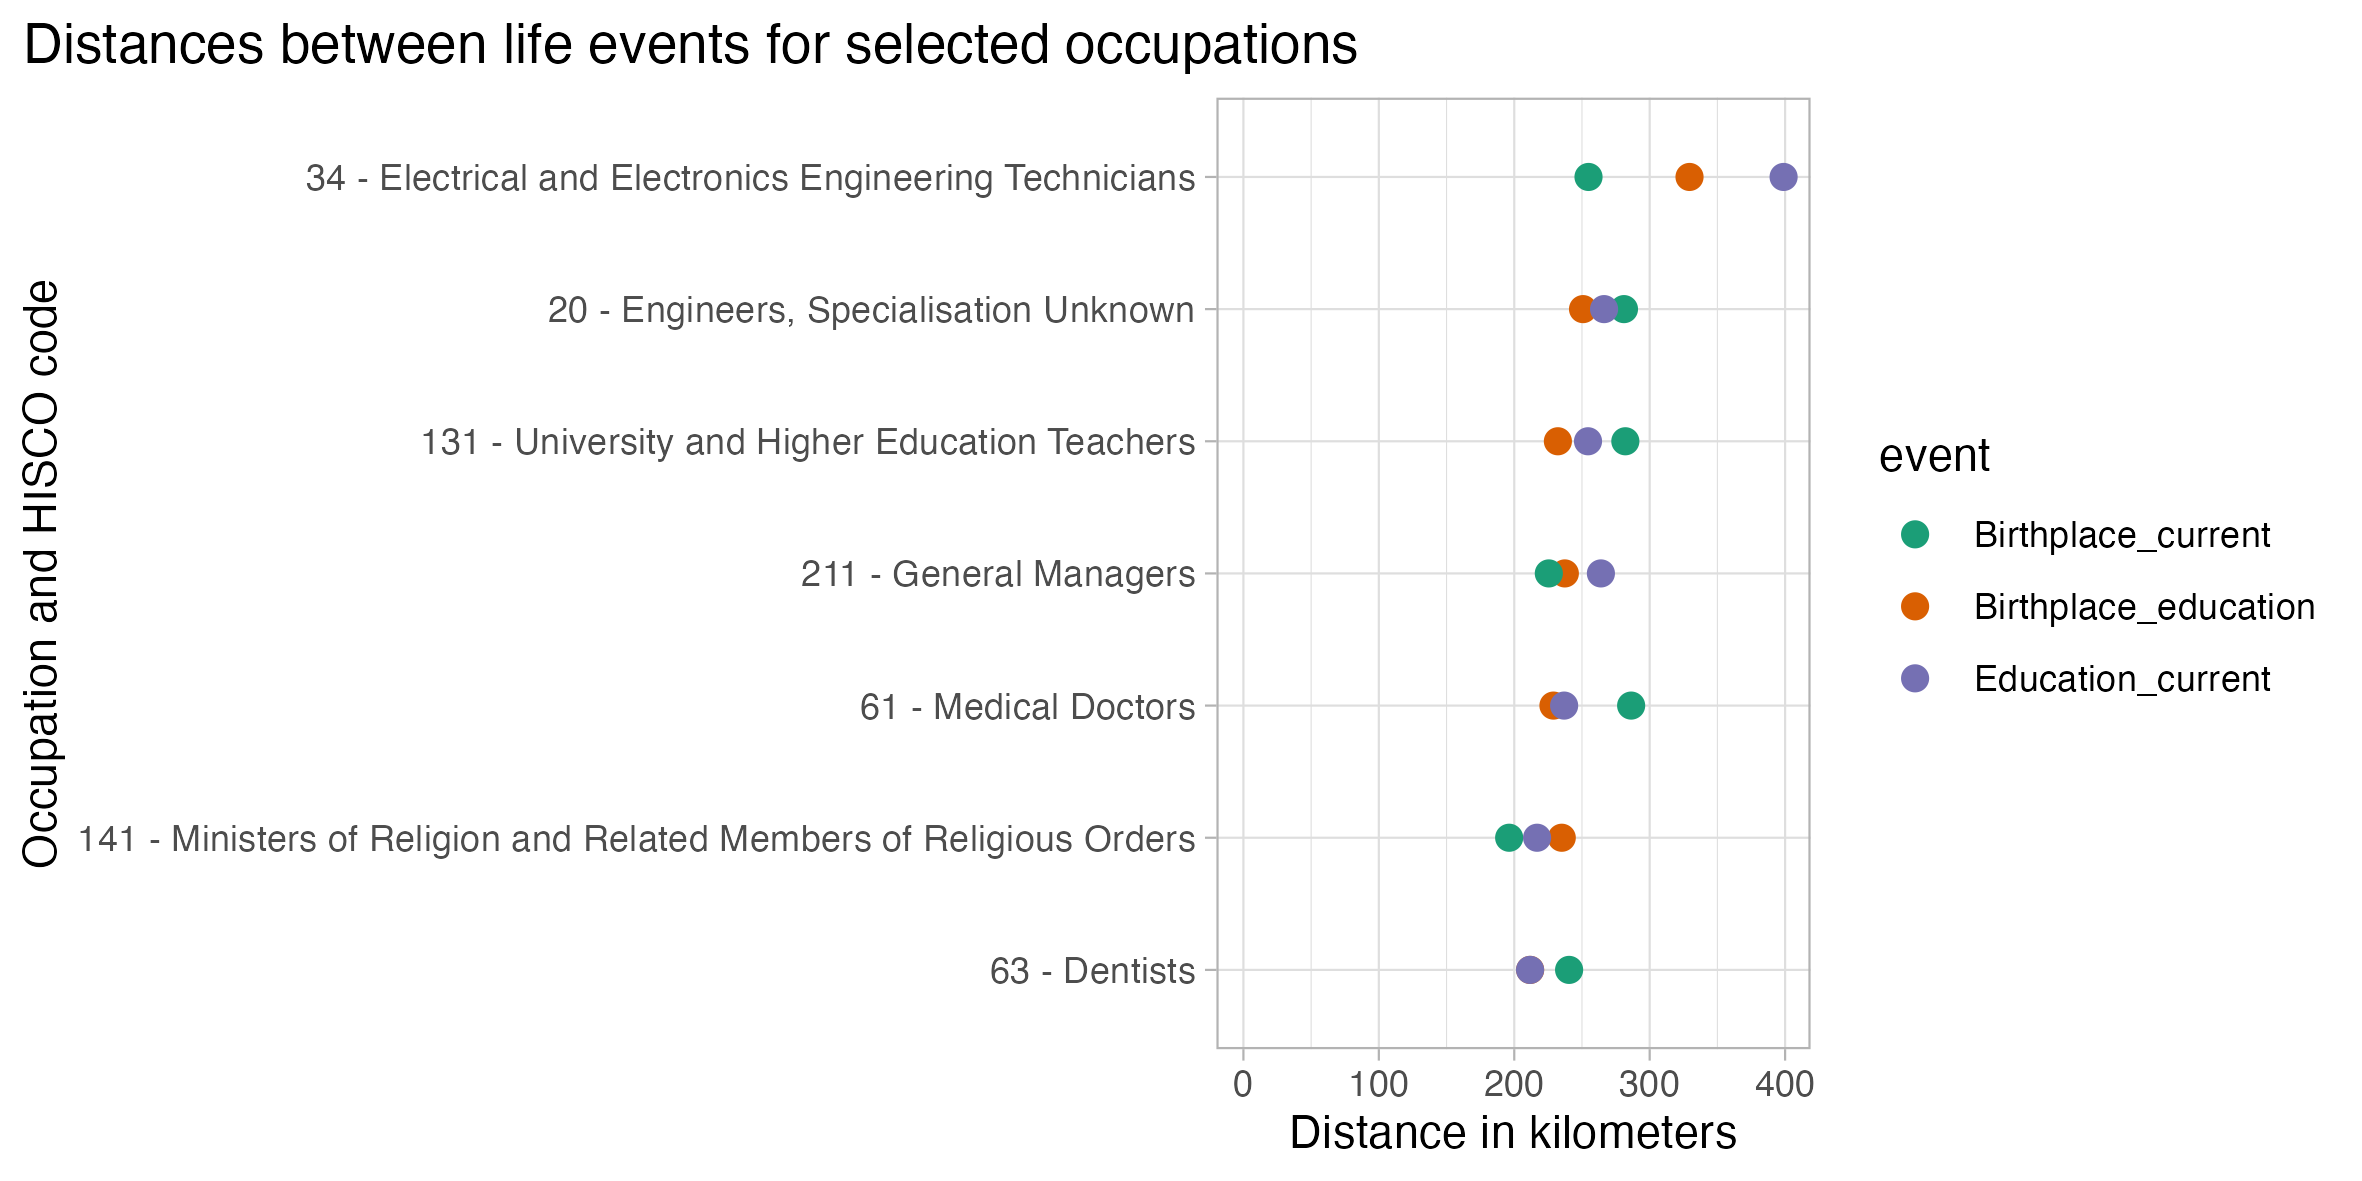
\includegraphics{assets/distances_comparison.png}

\hypertarget{appendix}{%
\subsection{Appendix}\label{appendix}}

Figure~\ref{fig-data-collection-process} outlines the data collection
process.

I scrape the book content from the \emph{Projekt Runeberg} website with
an HTML scraper (beautiful soup in python).

I split the records using regular expression in python, looking for
specific terms that begin and end the records in the dictionaries and
catalogue.

I augment the records with coordinates using the Google Maps Geocoding
API.

I store the data in JSON format, keeping the original text in the file
alongside the derived key value pairs.


\printbibliography[title=References]


\end{document}
